% This is the Reed College LaTeX thesis template. Most of the work
% for the document class was done by Sam Noble (SN), as well as this
% template. Later comments etc. by Ben Salzberg (BTS). Additional
% restructuring and APA support by Jess Youngberg (JY).
% Your comments and suggestions are more than welcome; please email
% them to cus@reed.edu
%
% See http://web.reed.edu/cis/help/latex.html for help. There are a
% great bunch of help pages there, with notes on
% getting started, bibtex, etc. Go there and read it if you're not
% already familiar with LaTeX.
%
% Any line that starts with a percent symbol is a comment.
% They won't show up in the document, and are useful for notes
% to yourself and explaining commands.
% Commenting also removes a line from the document;
% very handy for troubleshooting problems. -BTS

% As far as I know, this follows the requirements laid out in
% the 2002-2003 Senior Handbook. Ask a librarian to check the
% document before binding. -SN

%%
%% Preamble
%%
% \documentclass{<something>} must begin each LaTeX document
\documentclass[12pt,oneside]{reedthesis}
% Packages are extensions to the basic LaTeX functions. Whatever you
% want to typeset, there is probably a package out there for it.
% Chemistry (chemtex), screenplays, you name it.
% Check out CTAN to see: http://www.ctan.org/
%%
\usepackage{graphicx,latexsym}
\usepackage{amsmath}
\usepackage{amssymb,amsthm}
\usepackage{longtable,booktabs,setspace}
\usepackage{chemarr} %% Useful for one reaction arrow, useless if you're not a chem major
\usepackage[hyphens]{url}
% Added by CII
\usepackage{hyperref}
\usepackage{lmodern}
\usepackage{float}
\floatplacement{figure}{H}
% End of CII addition
\usepackage{rotating}
\linespread{1.25}
% Next line commented out by CII
%%% \usepackage{natbib}
% Comment out the natbib line above and uncomment the following two lines to use the new
% biblatex-chicago style, for Chicago A. Also make some changes at the end where the
% bibliography is included.
%\usepackage{biblatex-chicago}
%\bibliography{thesis}


% Added by CII (Thanks, Hadley!)
% Use ref for internal links
\renewcommand{\hyperref}[2][???]{\autoref{#1}}
\def\chapterautorefname{Chapter}
\def\sectionautorefname{Section}
\def\subsectionautorefname{Subsection}
% End of CII addition

% Added by CII
\usepackage{caption}
\captionsetup{width=5in}
% End of CII addition

% \usepackage{times} % other fonts are available like times, bookman, charter, palatino

% Syntax highlighting #22
  \usepackage{color}
  \usepackage{fancyvrb}
  \newcommand{\VerbBar}{|}
  \newcommand{\VERB}{\Verb[commandchars=\\\{\}]}
  \DefineVerbatimEnvironment{Highlighting}{Verbatim}{commandchars=\\\{\}}
  % Add ',fontsize=\small' for more characters per line
  \usepackage{framed}
  \definecolor{shadecolor}{RGB}{248,248,248}
  \newenvironment{Shaded}{\begin{snugshade}}{\end{snugshade}}
  \newcommand{\KeywordTok}[1]{\textcolor[rgb]{0.13,0.29,0.53}{\textbf{#1}}}
  \newcommand{\DataTypeTok}[1]{\textcolor[rgb]{0.13,0.29,0.53}{#1}}
  \newcommand{\DecValTok}[1]{\textcolor[rgb]{0.00,0.00,0.81}{#1}}
  \newcommand{\BaseNTok}[1]{\textcolor[rgb]{0.00,0.00,0.81}{#1}}
  \newcommand{\FloatTok}[1]{\textcolor[rgb]{0.00,0.00,0.81}{#1}}
  \newcommand{\ConstantTok}[1]{\textcolor[rgb]{0.00,0.00,0.00}{#1}}
  \newcommand{\CharTok}[1]{\textcolor[rgb]{0.31,0.60,0.02}{#1}}
  \newcommand{\SpecialCharTok}[1]{\textcolor[rgb]{0.00,0.00,0.00}{#1}}
  \newcommand{\StringTok}[1]{\textcolor[rgb]{0.31,0.60,0.02}{#1}}
  \newcommand{\VerbatimStringTok}[1]{\textcolor[rgb]{0.31,0.60,0.02}{#1}}
  \newcommand{\SpecialStringTok}[1]{\textcolor[rgb]{0.31,0.60,0.02}{#1}}
  \newcommand{\ImportTok}[1]{#1}
  \newcommand{\CommentTok}[1]{\textcolor[rgb]{0.56,0.35,0.01}{\textit{#1}}}
  \newcommand{\DocumentationTok}[1]{\textcolor[rgb]{0.56,0.35,0.01}{\textbf{\textit{#1}}}}
  \newcommand{\AnnotationTok}[1]{\textcolor[rgb]{0.56,0.35,0.01}{\textbf{\textit{#1}}}}
  \newcommand{\CommentVarTok}[1]{\textcolor[rgb]{0.56,0.35,0.01}{\textbf{\textit{#1}}}}
  \newcommand{\OtherTok}[1]{\textcolor[rgb]{0.56,0.35,0.01}{#1}}
  \newcommand{\FunctionTok}[1]{\textcolor[rgb]{0.00,0.00,0.00}{#1}}
  \newcommand{\VariableTok}[1]{\textcolor[rgb]{0.00,0.00,0.00}{#1}}
  \newcommand{\ControlFlowTok}[1]{\textcolor[rgb]{0.13,0.29,0.53}{\textbf{#1}}}
  \newcommand{\OperatorTok}[1]{\textcolor[rgb]{0.81,0.36,0.00}{\textbf{#1}}}
  \newcommand{\BuiltInTok}[1]{#1}
  \newcommand{\ExtensionTok}[1]{#1}
  \newcommand{\PreprocessorTok}[1]{\textcolor[rgb]{0.56,0.35,0.01}{\textit{#1}}}
  \newcommand{\AttributeTok}[1]{\textcolor[rgb]{0.77,0.63,0.00}{#1}}
  \newcommand{\RegionMarkerTok}[1]{#1}
  \newcommand{\InformationTok}[1]{\textcolor[rgb]{0.56,0.35,0.01}{\textbf{\textit{#1}}}}
  \newcommand{\WarningTok}[1]{\textcolor[rgb]{0.56,0.35,0.01}{\textbf{\textit{#1}}}}
  \newcommand{\AlertTok}[1]{\textcolor[rgb]{0.94,0.16,0.16}{#1}}
  \newcommand{\ErrorTok}[1]{\textcolor[rgb]{0.64,0.00,0.00}{\textbf{#1}}}
  \newcommand{\NormalTok}[1]{#1}

% To pass between YAML and LaTeX the dollar signs are added by CII
\title{analysis of flight data for weather dependant multiple execution
autonomous missions}
\author{Karl Uibo 153620IVEM}
% The month and year that you submit your FINAL draft TO THE LIBRARY (May or December)
\date{May 2018}
\division{School of Information Technologies}
\advisor{Supervisor: Olev Märtens}
\institution{tallinn university of technology}
\degree{Professor}
%If you have two advisors for some reason, you can use the following
% Uncommented out by CII
% End of CII addition

%%% Remember to use the correct department!
\department{Thomas Johann Seebeck Department of Electronics}
% if you're writing a thesis in an interdisciplinary major,
% uncomment the line below and change the text as appropriate.
% check the Senior Handbook if unsure.
%\thedivisionof{The Established Interdisciplinary Committee for}
% if you want the approval page to say "Approved for the Committee",
% uncomment the next line
%\approvedforthe{Committee}

% Added by CII
%%% Copied from knitr
%% maxwidth is the original width if it's less than linewidth
%% otherwise use linewidth (to make sure the graphics do not exceed the margin)
\makeatletter
\def\maxwidth{ %
  \ifdim\Gin@nat@width>\linewidth
    \linewidth
  \else
    \Gin@nat@width
  \fi
}
\makeatother

\renewcommand{\contentsname}{Table of Contents}
% End of CII addition

\setlength{\parskip}{0pt}

% Added by CII

\providecommand{\tightlist}{%
  \setlength{\itemsep}{0pt}\setlength{\parskip}{0pt}}

\Originality{
I hereby certify that I am the sole author of this thesis. All the used
materials, references to the literature and the work of others have been
referred to. This thesis has not been presented for examination anywhere
else.

~

Author: Karl Uibo

~

07.05.2018
}

\Annotatsioon{
Selles töös otsitakse lahendust probleemile, kuidas saavutada
autonoomset multirootori lennu missiooni nii, et lendude vahel ei peaks
ükski inimene sekkuma samal ajal maksimeerides lennuaega ja lennu
pikust. Senini on põhiliselt uuritud autopiloodi juht-algoritmide
efektiivsust ja on loodud ilmastiku ja sensori müra kindlamaid
algoritme. Selles töös vaadeldakse laiemat pilti, kus selleks, et
multirootorid saaksid olla tõeliselt autonoomsed ja võiksid pakuda
senini liialt kulukateks osutunud funktsionaalsusi. Selleks
analüüsitakse erinevaid võimalusi binaarsetest lennulogidest ühtse
andmestiku loomiseks. Vaadeldakse erinevaid faili tüüpe ning lõpuks
valitakse \emph{SQLite} andmebaas. Luuakse andmete mudel hoidmaks infot
logidest ja kirjutatakse kood \emph{python} keeles, mis loob nimetatud
andmebaasi. Andmebaasis olevate andmete analüüsi tulemusel leitakse
parameetrid, mille alusel on võimalik kogu andmebaasist välja
filtreerida andmed, mille abil on võimalik luua multirootori käitumise
mudel erinevatel lennu kiirustel õhu suhtes. Leitakse ka vajadus,
lendude pinge graafikuid analüüsides, et saavutada autonoomsus, mis
arvestab ilma tingitud muutustega autonoomsete missioonide vahel, on
tarvilik inteligentne kontroller, mis teaks autopiloodile anda infot aku
täituvusest. Kontroller peaks mõõtma ja arvestama aku temperatuuriga ja
jälgima aku degradatsiooni ajas ning kasutus kordadel. Lisaks peaks
kontroller väljastama unikaalse identifikaatori, et andmeanalüüsi
teostades oleks võimalik jälgida muutusi aku parameetrites.

See töö on kirjutatud Inglise keeles, on 35 lehekülge pikk, sisaldab 4
peatükki, 16 joonist ja 8 tabelit.
}

\Abstract{
This thesis explores how to achieve consecutive autonomous flights
without a pilots input. Previously the focus of research has been in
optimizing the flight characteristics of a multirotor but we take a
higher level approach to find the requirements needed to be able to
achieve fully autonomous flight with use cases in the industry.

We created \emph{python} code to import data from individual log files
into a database. An algorithm for filtering the database to find
necessary data to design a model of the flight behavior of an individual
multirotor is created. An analysis of voltage graphs of the available
flights were analyzed and a requirement for a smart controller in each
battery to monitor the state of charge, state of health and to identify
each battery is found.

This thesis is written in English and is 35 pages long, including 4
chapters, 16 figures and 8 tables.
}

\Abbrvs{
\begin{longtable}[]{@{}ll@{}}
\toprule
\begin{minipage}[b]{0.26\columnwidth}\raggedright\strut
\emph{Abbreviation}\strut
\end{minipage} & \begin{minipage}[b]{0.41\columnwidth}\raggedright\strut
\emph{Meaning}\strut
\end{minipage}\tabularnewline
\midrule
\endhead
\begin{minipage}[t]{0.26\columnwidth}\raggedright\strut
UAV\strut
\end{minipage} & \begin{minipage}[t]{0.41\columnwidth}\raggedright\strut
Unmanned Aerial Vehicle\strut
\end{minipage}\tabularnewline
\begin{minipage}[t]{0.26\columnwidth}\raggedright\strut
GPS\strut
\end{minipage} & \begin{minipage}[t]{0.41\columnwidth}\raggedright\strut
Global Positioning System\strut
\end{minipage}\tabularnewline
\begin{minipage}[t]{0.26\columnwidth}\raggedright\strut
GLONASS\strut
\end{minipage} & \begin{minipage}[t]{0.41\columnwidth}\raggedright\strut
Global Navigation Satellite System\strut
\end{minipage}\tabularnewline
\begin{minipage}[t]{0.26\columnwidth}\raggedright\strut
IMU\strut
\end{minipage} & \begin{minipage}[t]{0.41\columnwidth}\raggedright\strut
Inertial Measurement Unit\strut
\end{minipage}\tabularnewline
\begin{minipage}[t]{0.26\columnwidth}\raggedright\strut
GB\strut
\end{minipage} & \begin{minipage}[t]{0.41\columnwidth}\raggedright\strut
GigaByte - 1000\textsuperscript{3} bytes\strut
\end{minipage}\tabularnewline
\begin{minipage}[t]{0.26\columnwidth}\raggedright\strut
kB\strut
\end{minipage} & \begin{minipage}[t]{0.41\columnwidth}\raggedright\strut
kiloByte - 1000\textsuperscript{1} bytes\strut
\end{minipage}\tabularnewline
\begin{minipage}[t]{0.26\columnwidth}\raggedright\strut
MB\strut
\end{minipage} & \begin{minipage}[t]{0.41\columnwidth}\raggedright\strut
MegaByte - 1000\textsuperscript{2} bytes\strut
\end{minipage}\tabularnewline
\begin{minipage}[t]{0.26\columnwidth}\raggedright\strut
GCS\strut
\end{minipage} & \begin{minipage}[t]{0.41\columnwidth}\raggedright\strut
Ground Control Station\strut
\end{minipage}\tabularnewline
\begin{minipage}[t]{0.26\columnwidth}\raggedright\strut
CSV\strut
\end{minipage} & \begin{minipage}[t]{0.41\columnwidth}\raggedright\strut
Comma-Sepparated Values\strut
\end{minipage}\tabularnewline
\begin{minipage}[t]{0.26\columnwidth}\raggedright\strut
JSON\strut
\end{minipage} & \begin{minipage}[t]{0.41\columnwidth}\raggedright\strut
JavaScript Object Notation\strut
\end{minipage}\tabularnewline
\begin{minipage}[t]{0.26\columnwidth}\raggedright\strut
SQL\strut
\end{minipage} & \begin{minipage}[t]{0.41\columnwidth}\raggedright\strut
Structured Query Language\strut
\end{minipage}\tabularnewline
\begin{minipage}[t]{0.26\columnwidth}\raggedright\strut
DBMS\strut
\end{minipage} & \begin{minipage}[t]{0.41\columnwidth}\raggedright\strut
Database Management Systems\strut
\end{minipage}\tabularnewline
\begin{minipage}[t]{0.26\columnwidth}\raggedright\strut
PTZ camera\strut
\end{minipage} & \begin{minipage}[t]{0.41\columnwidth}\raggedright\strut
Point-Tilt-Zoom camera\strut
\end{minipage}\tabularnewline
\begin{minipage}[t]{0.26\columnwidth}\raggedright\strut
RTL\strut
\end{minipage} & \begin{minipage}[t]{0.41\columnwidth}\raggedright\strut
Return To Launch\strut
\end{minipage}\tabularnewline
\bottomrule
\end{longtable}
}

% End of CII addition
%%
%% End Preamble
%%
%

\usepackage{amsthm}
\newtheorem{theorem}{Theorem}[chapter]
\newtheorem{lemma}{Lemma}[chapter]
\newtheorem{corollary}{Corollary}[chapter]
\newtheorem{proposition}{Proposition}[chapter]
\newtheorem{conjecture}{Conjecture}[chapter]
\theoremstyle{definition}
\newtheorem{definition}{Definition}[chapter]
\theoremstyle{definition}
\newtheorem{example}{Example}[chapter]
\theoremstyle{definition}
\newtheorem{exercise}{Exercise}[chapter]
\theoremstyle{remark}
\newtheorem*{remark}{Remark}
\newtheorem*{solution}{Solution}
\begin{document}

% Everything below added by CII
  \maketitle
  \begin{originality}
    I hereby certify that I am the sole author of this thesis. All the used
    materials, references to the literature and the work of others have been
    referred to. This thesis has not been presented for examination anywhere
    else.
    
    ~
    
    Author: Karl Uibo
    
    ~
    
    07.05.2018
  \end{originality}
  \begin{abstract}
    This thesis explores how to achieve consecutive autonomous flights
    without a pilots input. Previously the focus of research has been in
    optimizing the flight characteristics of a multirotor but we take a
    higher level approach to find the requirements needed to be able to
    achieve fully autonomous flight with use cases in the industry.
    
    We created \emph{python} code to import data from individual log files
    into a database. An algorithm for filtering the database to find
    necessary data to design a model of the flight behavior of an individual
    multirotor is created. An analysis of voltage graphs of the available
    flights were analyzed and a requirement for a smart controller in each
    battery to monitor the state of charge, state of health and to identify
    each battery is found.
    
    This thesis is written in English and is 35 pages long, including 4
    chapters, 16 figures and 8 tables.
  \end{abstract}
  \begin{annotatsioon}
    Selles töös otsitakse lahendust probleemile, kuidas saavutada
    autonoomset multirootori lennu missiooni nii, et lendude vahel ei peaks
    ükski inimene sekkuma samal ajal maksimeerides lennuaega ja lennu
    pikust. Senini on põhiliselt uuritud autopiloodi juht-algoritmide
    efektiivsust ja on loodud ilmastiku ja sensori müra kindlamaid
    algoritme. Selles töös vaadeldakse laiemat pilti, kus selleks, et
    multirootorid saaksid olla tõeliselt autonoomsed ja võiksid pakuda
    senini liialt kulukateks osutunud funktsionaalsusi. Selleks
    analüüsitakse erinevaid võimalusi binaarsetest lennulogidest ühtse
    andmestiku loomiseks. Vaadeldakse erinevaid faili tüüpe ning lõpuks
    valitakse \emph{SQLite} andmebaas. Luuakse andmete mudel hoidmaks infot
    logidest ja kirjutatakse kood \emph{python} keeles, mis loob nimetatud
    andmebaasi. Andmebaasis olevate andmete analüüsi tulemusel leitakse
    parameetrid, mille alusel on võimalik kogu andmebaasist välja
    filtreerida andmed, mille abil on võimalik luua multirootori käitumise
    mudel erinevatel lennu kiirustel õhu suhtes. Leitakse ka vajadus,
    lendude pinge graafikuid analüüsides, et saavutada autonoomsus, mis
    arvestab ilma tingitud muutustega autonoomsete missioonide vahel, on
    tarvilik inteligentne kontroller, mis teaks autopiloodile anda infot aku
    täituvusest. Kontroller peaks mõõtma ja arvestama aku temperatuuriga ja
    jälgima aku degradatsiooni ajas ning kasutus kordadel. Lisaks peaks
    kontroller väljastama unikaalse identifikaatori, et andmeanalüüsi
    teostades oleks võimalik jälgida muutusi aku parameetrites.
    
    See töö on kirjutatud Inglise keeles, on 35 lehekülge pikk, sisaldab 4
    peatükki, 16 joonist ja 8 tabelit.
  \end{annotatsioon}
  \begin{abbrvs}
    \begin{longtable}[]{@{}ll@{}}
    \toprule
    \begin{minipage}[b]{0.26\columnwidth}\raggedright\strut
    \emph{Abbreviation}\strut
    \end{minipage} & \begin{minipage}[b]{0.41\columnwidth}\raggedright\strut
    \emph{Meaning}\strut
    \end{minipage}\tabularnewline
    \midrule
    \endhead
    \begin{minipage}[t]{0.26\columnwidth}\raggedright\strut
    UAV\strut
    \end{minipage} & \begin{minipage}[t]{0.41\columnwidth}\raggedright\strut
    Unmanned Aerial Vehicle\strut
    \end{minipage}\tabularnewline
    \begin{minipage}[t]{0.26\columnwidth}\raggedright\strut
    GPS\strut
    \end{minipage} & \begin{minipage}[t]{0.41\columnwidth}\raggedright\strut
    Global Positioning System\strut
    \end{minipage}\tabularnewline
    \begin{minipage}[t]{0.26\columnwidth}\raggedright\strut
    GLONASS\strut
    \end{minipage} & \begin{minipage}[t]{0.41\columnwidth}\raggedright\strut
    Global Navigation Satellite System\strut
    \end{minipage}\tabularnewline
    \begin{minipage}[t]{0.26\columnwidth}\raggedright\strut
    IMU\strut
    \end{minipage} & \begin{minipage}[t]{0.41\columnwidth}\raggedright\strut
    Inertial Measurement Unit\strut
    \end{minipage}\tabularnewline
    \begin{minipage}[t]{0.26\columnwidth}\raggedright\strut
    GB\strut
    \end{minipage} & \begin{minipage}[t]{0.41\columnwidth}\raggedright\strut
    GigaByte - 1000\textsuperscript{3} bytes\strut
    \end{minipage}\tabularnewline
    \begin{minipage}[t]{0.26\columnwidth}\raggedright\strut
    kB\strut
    \end{minipage} & \begin{minipage}[t]{0.41\columnwidth}\raggedright\strut
    kiloByte - 1000\textsuperscript{1} bytes\strut
    \end{minipage}\tabularnewline
    \begin{minipage}[t]{0.26\columnwidth}\raggedright\strut
    MB\strut
    \end{minipage} & \begin{minipage}[t]{0.41\columnwidth}\raggedright\strut
    MegaByte - 1000\textsuperscript{2} bytes\strut
    \end{minipage}\tabularnewline
    \begin{minipage}[t]{0.26\columnwidth}\raggedright\strut
    GCS\strut
    \end{minipage} & \begin{minipage}[t]{0.41\columnwidth}\raggedright\strut
    Ground Control Station\strut
    \end{minipage}\tabularnewline
    \begin{minipage}[t]{0.26\columnwidth}\raggedright\strut
    CSV\strut
    \end{minipage} & \begin{minipage}[t]{0.41\columnwidth}\raggedright\strut
    Comma-Sepparated Values\strut
    \end{minipage}\tabularnewline
    \begin{minipage}[t]{0.26\columnwidth}\raggedright\strut
    JSON\strut
    \end{minipage} & \begin{minipage}[t]{0.41\columnwidth}\raggedright\strut
    JavaScript Object Notation\strut
    \end{minipage}\tabularnewline
    \begin{minipage}[t]{0.26\columnwidth}\raggedright\strut
    SQL\strut
    \end{minipage} & \begin{minipage}[t]{0.41\columnwidth}\raggedright\strut
    Structured Query Language\strut
    \end{minipage}\tabularnewline
    \begin{minipage}[t]{0.26\columnwidth}\raggedright\strut
    DBMS\strut
    \end{minipage} & \begin{minipage}[t]{0.41\columnwidth}\raggedright\strut
    Database Management Systems\strut
    \end{minipage}\tabularnewline
    \begin{minipage}[t]{0.26\columnwidth}\raggedright\strut
    PTZ camera\strut
    \end{minipage} & \begin{minipage}[t]{0.41\columnwidth}\raggedright\strut
    Point-Tilt-Zoom camera\strut
    \end{minipage}\tabularnewline
    \begin{minipage}[t]{0.26\columnwidth}\raggedright\strut
    RTL\strut
    \end{minipage} & \begin{minipage}[t]{0.41\columnwidth}\raggedright\strut
    Return To Launch\strut
    \end{minipage}\tabularnewline
    \bottomrule
    \end{longtable}
  \end{abbrvs}
  \hypersetup{linkcolor=black}
  \setcounter{tocdepth}{2}
  \tableofcontents

  \listoffigures

  \listoftables

\mainmatter % here the regular arabic numbering starts
\pagestyle{plain} % turns page numbering back on

\chapter*{Introduction}\label{introduction}
\addcontentsline{toc}{chapter}{Introduction}

Currently the autonomy of multirotor aircraft is limited to single
flights. A mission can be made that traverses a given path and points
its camera at points of interest. The current technology lets the pilot
assign the speed of flight during the traversal of the mission. Eli Ltd
has developed a technology that they call \emph{nests}. With this
technology the batteries of a multirotor can be recharged and swapped
for charged ones. This creates the possibility to create missions that
are automatic and require no input from a pilot. Due to the dynamic
nature of weather the flight speeds of the mission need to be changed.
By changing the speeds safety and higher operational ability is
achieved. Current technology does not dynamically change the mission
parameters to fit the weather conditions.

This thesis does not concern itself with use cases where high
situational awareness is needed such as detecting objects in video,
tracking objects in video, dynamically generating new missions given
external stimulus. Instead use cases that use missions that follow a
preplanned path are discussed. Such use cases are area surveillance
missions for securing a perimeter of a secure site or autonomous patrol
of a segment of a countries border.

More concretely in this thesis the library of binary flight logs of Eli
Ltd is taken and used to build a database for further analysis. In the
first chapter we survey the state of the art. The second chapter
discusses the intricacies of piloting an unmanned aerial multirotor
vehicle. In the third chapter various file formats are analyzed and
chosen from to be used as storage for the database. Furthermore the
analysis prerequisites are discussed and the database schema is designed
accordingly. The schema is then used in the \emph{python} code created
by the thesis author to translate the binary flight logs into a
\emph{SQLite} database. In the following chapter initial analysis is
conducted on the data. The goal of which is to find the relevant data to
model the multirotor behavior in different conditions and requirements
for the model to be used in practice.

\chapter{State of the art}\label{state}

A multirotor UAV may carry different payloads for different use cases
but predominantly the payload is a video or photo camera. The video and
photos can be used for 3D mapping, search and rescue operations,
inspecting power lines, surveillance, inspecting wind turbine structural
integrity, counting deer in woods or simply capturing cinematic footage
to name a few. However the act of piloting itself is secondary to the
goal. The act of piloting is necessary to gather data with the payload.
A pilot needs to have certain skills and training to be able to safely
operate an aerial vehicle. The cost of hiring a pilot can be much higher
than the operational costs of the UAV and payload combined. Thus
companies across the globe look to simplify the piloting.

In movie industry camera drones are used with two people. One person to
pilot the multirotor and one person to manipulate the camera. This has
the overhead of hiring two people and the multirotor and the expensive
payload. For the high-end movie industry this is fine. Where this
overhead becomes prohibitive is in the industrial applications. To
inspect power lines at least one person is needed to do the piloting and
directing of the camera. The video analysis can be done during the
flight or later. To keep the needs of man power to a minimum the
operator needs to be able to operate the multirotor as well as the
camera and know enough of the power lines to analyse the video feed.
Another option is to have two people - one to pilot and film and a
second one to do the analysis. The operator however might not film the
correct parts for the analyst to do his job. Thus introducing the risk
that the collected data is unusable. In the case of power lines not only
a single pylon needs to be inspected, rather several hundred kilometers
worth need to be assessed at a time. Having a single person drive to
each location to fly a multirotor would take a very long time for a
single person and as the person needs to be highly trained the process
would become prohibitively expensive. This problem is smaller when it
comes to tele-communications companies as they have single cell towers
which allays need to be inspected one at a time. For the energy sector a
multirotor is prohibitively expensive and not because of the device
costs but rather the manpower costs.

The energy sector could use multirotors, but they have a more cost
effective way of detecting faults. The method involves renting a full
size helicopter with a pilot and fitting it with a expensive camera and
camera operator to fly over the power lines at the right angles to later
analyse the photos or video taken. This has a higher chance of missing
faults but compared to multirotors is cheaper alternative.

Automating the missions to inspect power lines or cell towers requires
high intelligence on the part of the autopilot and will not be assessed
in this thesis. Instead search and rescue missions and surveillance
missions are assessed. These missions have the potential to be
simplified to the point where additional training on the part of the
pilot is not needed.
\begin{figure}
\centering
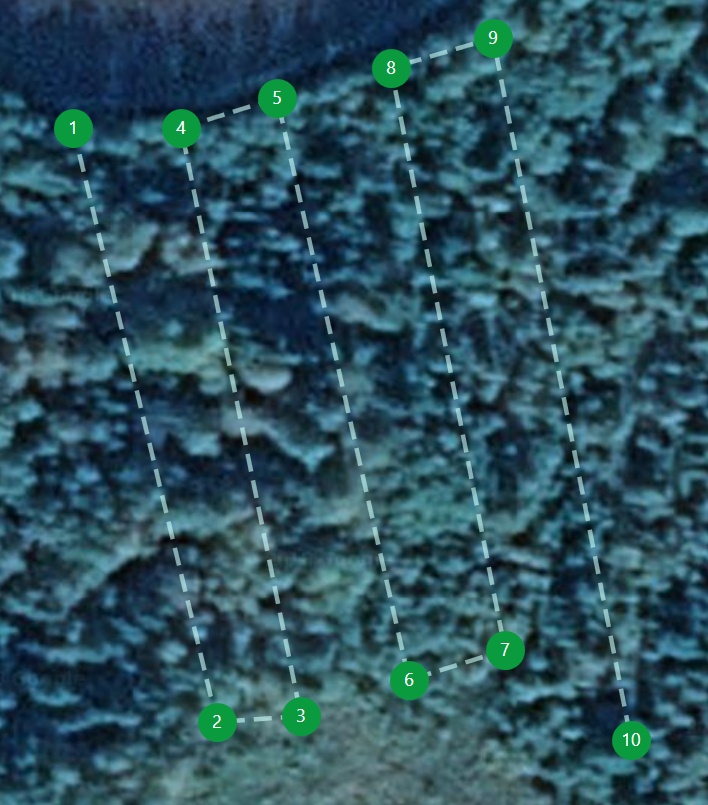
\includegraphics{./figure/scanningMission.PNG}
\caption[\label{fig:scanning}Search and rescue
mission.]{\label{fig:scanning}Search and rescue mission.\footnotemark{}}
\end{figure}
\footnotetext{Image captured from Elix software made by Eli Ltd.}

To find a person lost in woods a mission such as seen on figure
\ref{fig:scanning} is used. To execute such a mission the pilot needs to
take into account several variables such as wind speed and battery
condition. A naive simplification to piloting can be made by limiting
the maximum disturbance (wind) allowed by forcibly landing when such
disturbance is detected. This sets a hard limit to the conditions an
unskilled pilot can fly in. By enforcing such a limit the risk of
failure can be minimized and the producer of the multirotor would feel a
lot better about their product. A skilled pilot however would be able to
fly and potentially save someones life in that situation. A better
approach is needed.
\begin{figure}
\centering
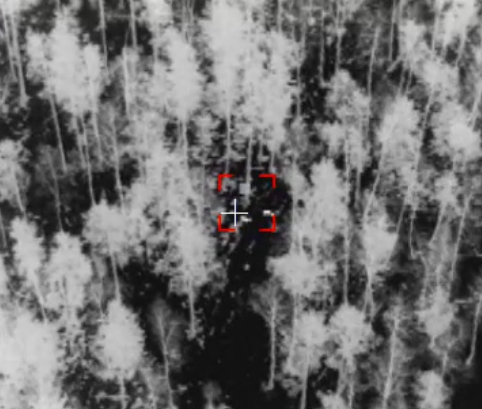
\includegraphics{./figure/twoDeer.PNG}
\caption[\label{fig:twoDeer}Heat signals of two deer in the
woods.]{\label{fig:twoDeer}Heat signals of two deer in the
woods.\footnotemark{}}
\end{figure}
\footnotetext{Source: Eli Ltd photo repository.}
\begin{figure}
\centering
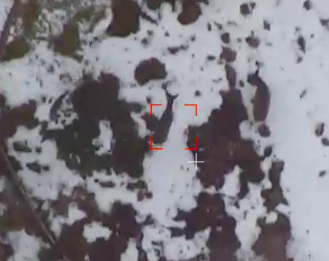
\includegraphics{./figure/deer.PNG}
\caption[\label{fig:deer}A deer in the woods.]{\label{fig:deer}A deer in the
woods.\footnotemark{}}
\end{figure}
\footnotetext{Source: Eli Ltd photo repository.}

Area surveillance requires an automated mission that allows for
specification of the camera direction and angle. A mission to survey the
fences of a military compound would have to include waypoints that
specify the locations the multirotor flies to and the locations or
directions the multirotor camera is turned to while flying. While
building such a mission takes some knowledge of the software the actual
mission takes no input from a pilot (unless desired) and can be used the
same way a regular camera video is used. When the viewer of the video
feed spots that something is wrong, the multirotor could be set to
manual control mode to be used as flying camera in a similar fashion to
PTZ cameras. Such systems could be used instead of stationary cameras in
cases where the areas are to big to have stationary camera
infrastructure or change rapidly. Given the naive solution to dealing
with different weather conditions outlined above would leave the area
vulnerable every time the weather conditions exceed the piloting
abilities of an untrained pilot. To remedy this the autopilot needs to
be able to adjust to the weather conditions in the same way an
experienced pilot would.

\chapter{Piloting a multirotor UAV}\label{piloting}

During the flight of a multirotor UAV several things happen at once.
Firstly the UAV fights against gravity to keep itself at the desired
height. Secondly it has to follow the orders of the pilot - fly as
desired. Thirdly the UAV also fights against the wind. This combination
of three forces means that the system is highly dynamic. While the
gravity is constant, the desires of the pilot change as well as the
wind.

The pilot can be in control largely by two ways:
\begin{enumerate}
\def\labelenumi{\arabic{enumi}.}
\tightlist
\item
  Manual control via analog controllers
\item
  Automatic flight mode via commands
\end{enumerate}
During manual mode the UAV is directed by analog controllers that give
it some sort of continuous input signal to adjust the throttle of the
four motors. Changing the throttle results in either tilting of the
aircraft or changing of its altitude or both. Different vendors offer
differing levels of control. In \emph{arducopter}\footnote{A
  full-featured, open-source multicopter UAV controller firmware.}
firmware there is \emph{stabilize} mode that allows the pilot to fly
manually, but the platform self-levels the roll and pitch axis. If the
pilot releases the controls the UAV falls to the ground. In \emph{DJI}
Phantom 4\footnote{A Chinese producer of multirotor UAV's. Phantom 4 is
  a successful commercially available multirotor platform.} there are
modes such as \emph{Position Mode} which uses GPS and GLONASS satellite
positioning where releasing the controls results in the platform
remaining stationary in air even in windy conditions. A similar mode
exists in arducopter called \emph{loiter}. In this some simplification
of piloting can be seen. The autopilot is there to remove a component of
skills needed for successful piloting. In these modes the pilot is in
control of the speed of flight and is in effect compensating for the
effects of wind when flying in some direction. While staying still the
GPS location is used to stay still.

Both \emph{arducopter} and \emph{DJI} have automatic flight modes where
the multirotor flies according to a pre-programmed mission. The missions
are user specified by global x/y coordinates, height values and the
speed of flight between points. The multirotor autonomously attempts to
fly through given mission points at the given height and speed. During
such a flight the multirotor automatically compensates for wind. In the
case of \emph{DJI} a wind warning is given at 6 m/s winds and high wind
warning at 9 m/s. \emph{Arducopter} does not report the wind and leaves
everything to the pilot.

The complications of piloting due to wind are numerous and we will look
at a few of them.
\begin{enumerate}
\def\labelenumi{\arabic{enumi}.}
\item
  Angles of the multirotor when stationary (\emph{loiter} mode) reflect
  wind direction.
\item
  Current draw from the battery increases.
\item
  Vibrations aboard the multirotor increase.
\end{enumerate}
When the aircraft is stationary above ground the wind causes it to tilt
into the wind. In the reference frame of air, the multirotor is flying
at the speed of the wind and in opposite direction, to, in the reference
frame of the ground, remain stationary. Looking at the angles there is
no difference between standing still in 5 m/s wind and flying in some
direction with the speed of 5 m/s in windless weather.
\begin{figure}
\centering
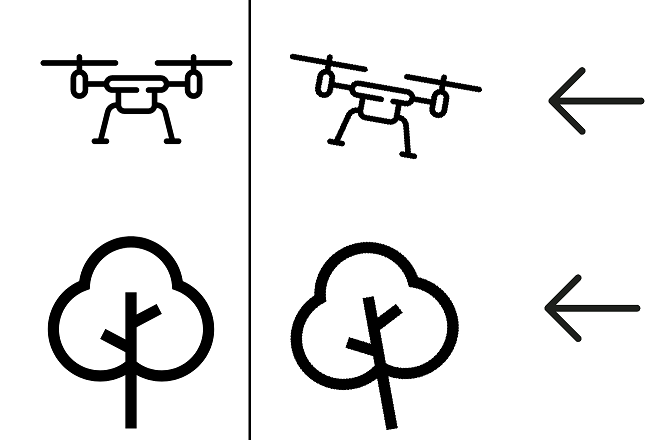
\includegraphics{./figure/wind.PNG}
\caption[\label{fig:wind}Stationary multirotor without and with
wind.]{\label{fig:wind}Stationary multirotor without and with
wind.\footnotemark{}}
\end{figure}
\footnotetext{Arrow icon made by
  \url{https://www.flaticon.com/authors/lyolya}, multirotor and tree
  icon made by \url{https://www.flaticon.com/authors/freepik} from
  www.flaticon.com}

Secondly, when flying against the wind, the current draw increases to
match the increased power required to stay airborne. From the power
consumption point of view there is no difference in flying 5 m/s in some
direction to standing still in 5 m/s wind.

Thirdly the vibrations aboard the aircraft increase. This can cause
trouble for the flight controller as the output of the IMU's becomes
noisy. Since the flight controller calculates the outputs of the motors
using various sensors and among them IMU's, high vibration may cause the
flight controller to be unable to determine its attitude and as a result
cause the aircraft to loose control and crash. In this thesis we will
look mainly at the first two effects.

To operate a multirotor manually the pilot needs to take those effects
into account and keep their eyes on the readings of those parameters.
The simplified flight modes such as \emph{loiter} take most of the skill
needed to pilot by implementing features on the autopilot. Several
control algorithms have been developed, such as the widely used
\emph{proportional} \emph{integral} \emph{derivative} algorithm,
\emph{cascaded} \emph{linear} \emph{proportional} \emph{integral}
\emph{derivative}\footnote{Yu, Yang, Wang, Li, \& Li (2015)} algorithm
or the newer \emph{incremental} \emph{nonlinear} \emph{dynamic}
\emph{inversion}\footnote{Smeur, Croon, \& Chu (2018)} algorithm. These
algorithms optimize for the stability of the flight reducing the need
for the pilot to do it by hand but higher level algorithms are still at
the level of naive implementations for features such as optimizing for
flight time or distance or speed, optimizing for safe return to start.
These features are of critical importance for achieving full autonomy in
some scenarios.

For safety both \emph{arducopter} and \emph{DJI} use fail-safe modes to
guarantee that the multirotor has enough power left to reach the
take-off location. A naive approach that \emph{arducopter} employs is to
look at the battery voltage and at a fixed point start flying back. This
safety behavior can be triggered in both manual control mode and
automatic mission mode. This approach has to take into account the worst
case scenario of flying against the wind a long distance to make sure
the multirotor makes it back. This leave a portion of the available
power in the battery as a buffer reserve. A smarter fail-safe would also
take into account the distance from the starting location to scale the
value where the fail-safe is triggered. This helps reduce the buffer
energy requirement. To further reduce the energy left in the buffer the
fail-safe would also need to adjust for the weather conditions. If the
starting location is down wind then much less energy is needed than when
the return home trip is taken against the wind. To achieve this type of
smart fail-safe functionality the autopilot needs to be aware of two
things:
\begin{enumerate}
\def\labelenumi{\arabic{enumi}.}
\item
  The wind parameters - strength and direction.
\item
  The battery state - how much energy is left in the battery.
\end{enumerate}
To find the wind parameters a fusion of an on-board wind sensor and
magnetometer could be used. An on board wind sensor has been used to
measure winds in wind farms to model airflow\footnote{Palomaki, Rose,
  Bossche, Sherman, \& Wekker (2017)}. The multirotors that Eli Ltd
produces do not have on-board wind sensors. As there is no difference
between a multirotor flying at a fixed speed in windless conditions or
staying stationary when the wind is equal to that of the previous
example. Therefore a model of behavior could be created given flight
data where wind is minimal or zero. In the next chapter creating a
database to use in modelling is discussed and the code to do so is
created.

Given a database of flight logs the behavior of batteries can be
analyzed. This is done later in this thesis.

\chapter{Database generation}\label{dbs}

\section{Inital data}\label{inital-data}

Eli Ltd collects the binary flight logs that are saved by arducopter
firmware aboard the multirotor platform. The binary files contain
\emph{MAVLink} protocol packets. \emph{MAVLink} stands for \emph{Micro
Air Vehicle Message Marshalling Library}.
\begin{quote}
\emph{MAVLink is a very lightweight, header-only message library for
communication between drones and/or ground control stations. It consists
primarily of message-set specifications for different systems
(``dialects'') defined in XML files, and Python tools that convert these
into appropriate source code for supported languages.}\footnote{ArduCopter
  team (n.d.-b)}
\end{quote}
Not all possible messages that the autopilot generates are sent to the
GCS. It is configurable which packets are saved, which are sent to the
GCS and which are dropped. In general the GCS receives some subset of
all messages that is important for operating the multirotor. In the logs
a bigger subset is recorded. For the logs present most important
messages and communications are saved but extremely high resolution data
is not saved. As such over a thousand logs have been collected. The
total number of binary logs available is 1363 and amount to 57.2 GB of
data. This would average 41966 KB per log. Among them are logs that are
not actual flights but rather tests on the bench. These logs inflate the
number of logs available. Some logs do contain the highest amounts of
data and can be several hundred MB large and thus inflate the average. A
normal flight can be expected to be between 4 to 100 MB's. An average
40+ minute flight is expected to be over 40 MB.

\hypertarget{choosing-the-output-data-type}{\section{Choosing the output
data type}\label{choosing-the-output-data-type}}

In this thesis \emph{R}\footnote{R Development Core Team (2004)}
programming language is used for data analysis. \emph{R} is a language
and environment for statistical computing and graphics. As it is open
source no licences are required to set it up and use. This brings
statistical computing and data science to the hands of everyone
interested in the topic and avoids expensive mathematics suites.

The binary data in the log files is not readily accessible from
\emph{R}. As a result it is necessary to convert the data to some other
format. The \emph{pymavlink} project - a \emph{python} implementation of
MAVLink protocol\footnote{ArduPilot team (n.d.-b)} - has a few tools
that do just that. First of the options is to convert the log into a
CSV\footnote{Comma separated values file is a text file where a comma is
  used to separate values.} file. \emph{Mavlogdump.py}\footnote{ArduPilot
  team (n.d.-a)} is the tool available for conversion. With CSV files
comes a caveat - you may only export one message type at a time. This is
to be expected since the the CSV files separate table columns with
commas and the log files have message types with different lengths of
columns. Example lines of CSV file taken from a flight log containing
NTUN packets.
\begin{verbatim}
timestamp,TimeUS,DPosX,DPosY,PosX,PosY,DVelX,DVelY,VelX,VelY,DAccX,...
1521817093.27547407,688646373,-489.633148193,86.0853424072...
1521817093.37760210,688748501,-489.633148193,86.0853424072...
1521817093.47829199,688849191,-489.633148193,86.0853424072...
\end{verbatim}
In \emph{R} it is very simple to import CSV files and this at first
seemed a viable candidate file type for storage. However since there are
many different types of messages, each log would in turn be converted to
as many CSV files. Potentially leaving us with tens of thousands of
files. This means \emph{R} would have to import the relevant files one
by one and processing them. With thousands of files to import the
analysis time would be negatively impacted as the data import poses an
overhead.

Another option is to use JSON\footnote{Crockford (n.d.)}. JSON is a
data-interchange format designed to be easily read and written by humans
as well as to be easily parsed and generated by machines. There are two
structures in JSON:
\begin{itemize}
\item
  A collection of name/value pairs.
\item
  An ordered list of values.
\end{itemize}
Both are familiar to programmers using the \emph{C}-family languages.
Both can be seen in the following example:
\begin{Shaded}
\begin{Highlighting}[]
\NormalTok{\{}\StringTok{"menu"}\OperatorTok{:}\StringTok{ }\NormalTok{\{}
  \StringTok{"id"}\OperatorTok{:}\StringTok{ "file"}\NormalTok{,}
  \StringTok{"value"}\OperatorTok{:}\StringTok{ "File"}\NormalTok{,}
  \StringTok{"popup"}\OperatorTok{:}\StringTok{ }\NormalTok{\{}
    \StringTok{"menuitem"}\OperatorTok{:}\StringTok{ }\NormalTok{[}
\NormalTok{      \{}\StringTok{"value"}\OperatorTok{:}\StringTok{ "New"}\NormalTok{, }\StringTok{"onclick"}\OperatorTok{:}\StringTok{ "CreateNewDoc()"}\NormalTok{\},}
\NormalTok{      \{}\StringTok{"value"}\OperatorTok{:}\StringTok{ "Open"}\NormalTok{, }\StringTok{"onclick"}\OperatorTok{:}\StringTok{ "OpenDoc()"}\NormalTok{\},}
\NormalTok{      \{}\StringTok{"value"}\OperatorTok{:}\StringTok{ "Close"}\NormalTok{, }\StringTok{"onclick"}\OperatorTok{:}\StringTok{ "CloseDoc()"}\NormalTok{\}}
\NormalTok{    ]}
\NormalTok{  \}}
\NormalTok{\}\}}
\end{Highlighting}
\end{Shaded}
Two consecutive entries from the binary log converted to json format
using \emph{mavlogdump.py} look like this:
\begin{Shaded}
\begin{Highlighting}[]
\NormalTok{\{}\StringTok{"meta"}\OperatorTok{:}\StringTok{ }\NormalTok{\{}
    \StringTok{"timestamp"}\OperatorTok{:}\StringTok{ }\FloatTok{1521817579.039407}\NormalTok{, }
    \StringTok{"type"}\OperatorTok{:}\StringTok{ "PIDP"}
\NormalTok{  \}, }
  \StringTok{"data"}\OperatorTok{:}\StringTok{ }\NormalTok{\{}
    \StringTok{"D"}\OperatorTok{:}\StringTok{ }\OperatorTok{-}\FloatTok{0.0005177092389203608}\NormalTok{, }
    \StringTok{"TimeUS"}\OperatorTok{:}\StringTok{ }\DecValTok{1174410306}\NormalTok{, }
    \StringTok{"I"}\OperatorTok{:}\StringTok{ }\FloatTok{0.0324220173060894}\NormalTok{, }
    \StringTok{"AFF"}\OperatorTok{:}\StringTok{ }\FloatTok{0.0}\NormalTok{, }
    \StringTok{"Des"}\OperatorTok{:}\StringTok{ }\OperatorTok{-}\FloatTok{0.012198338285088539}\NormalTok{, }
    \StringTok{"P"}\OperatorTok{:}\StringTok{ }\OperatorTok{-}\FloatTok{0.005622388795018196}\NormalTok{, }
    \StringTok{"FF"}\OperatorTok{:}\StringTok{ }\OperatorTok{-}\FloatTok{0.0}
\NormalTok{  \}}
\NormalTok{\}}
\NormalTok{\{}\StringTok{"meta"}\OperatorTok{:}\StringTok{ }\NormalTok{\{}
    \StringTok{"timestamp"}\OperatorTok{:}\StringTok{ }\FloatTok{1521817579.039419}\NormalTok{, }
    \StringTok{"type"}\OperatorTok{:}\StringTok{ "PIDY"}
\NormalTok{  \}, }
  \StringTok{"data"}\OperatorTok{:}\StringTok{ }\NormalTok{\{}
    \StringTok{"D"}\OperatorTok{:}\StringTok{ }\OperatorTok{-}\FloatTok{0.0}\NormalTok{, }
    \StringTok{"TimeUS"}\OperatorTok{:}\StringTok{ }\DecValTok{1174410318}\NormalTok{, }
    \StringTok{"I"}\OperatorTok{:}\StringTok{ }\OperatorTok{-}\FloatTok{0.08129391074180603}\NormalTok{, }
    \StringTok{"AFF"}\OperatorTok{:}\StringTok{ }\FloatTok{0.0}\NormalTok{, }
    \StringTok{"Des"}\OperatorTok{:}\StringTok{ }\FloatTok{0.006200382951647043}\NormalTok{, }
    \StringTok{"P"}\OperatorTok{:}\StringTok{ }\FloatTok{0.008107485249638557}\NormalTok{, }
    \StringTok{"FF"}\OperatorTok{:}\StringTok{ }\FloatTok{0.0}
\NormalTok{  \}}
\NormalTok{\}}
\end{Highlighting}
\end{Shaded}
\emph{R} has libraries to deal with JSON data. Such as
\emph{jsonlite}\footnote{Ooms (2014)} and \emph{rjson}\footnote{Couture-Beil
  (2014)}. As with CSV, JSON files need to be imported one by one,
analyzed and unloaded. This has considerable overhead. Further more an
output file from a 47.6 MB log file becomes 649.8 MB. That is an
increase of size of thirteen times! The library of logs that is 57.2 GB
becomes 743.6 GB of JSON data as a result. At least there are an order
of magnitude lower amount of files.

The final option to consider is \emph{SQLite}\footnote{(``About
  sqlite,'' n.d.)}. \emph{SQLite} is a \emph{SQL} database engine that
is self-contained and serverless. It is designed to be \emph{SQL}
database, but without concerning itself with a server process and user
management and other common \emph{SQL} attributes. As such its designed
to be a competitor to both JSON and CSV. The benefit of \emph{SQLite} is
that it can be used by various third party programs and programming
languages. \emph{Python} and \emph{Tcl} have \emph{SQLite} built in. Raw
data can be imported from CSV files and the data can be compressed to
similar sizes to \emph{Zip} files. Since the database is a single file
it can easily be written to a USB memory stick or with smaller databases
emailed to a colleague directly. Given some understanding of \emph{SQL}
\emph{SQLite} offers an easy to use database.

\emph{R} language has adapters to connect to \emph{SQL} databases such
as \emph{RODBC}\footnote{Ripley \& Lapsley (2017)},
\emph{RJDBC}\footnote{Urbanek (2018)}, \emph{bigrquery}\footnote{Wickham
  (2018)} and many others among which is \emph{RSQLite}\footnote{Müller,
  Wickham, James, \& Falcon (2017)}. \emph{RSQLite} embeds the
\emph{SQLite} database engine in \emph{R}, providing a
\emph{DBI}\footnote{R Special Interest Group on Databases (R-SIG-DB),
  Wickham, \& Müller (2018)}-compliant interface. \emph{DBI} is an
\emph{R} package that defines a common interface between \emph{R} and
database management systems (\emph{DBMS}). With \emph{RSQLite} package
it is possible to directly manipulate data in \emph{SQLite} database.

\section{Tidy data}\label{tidy-data}

Tidy data is a set of principles that help organize data in data sets.
This helps make data cleaning easier and faster by not having to start
from scratch every time. Another benefit of tidy data is that it is
easier to design data analysis tools which can assume that the data
input is always tidy. Both benefits help the data analyser to focus on
the underlying problem rather than managing data half the time\footnote{Wickham
  (2014)}.
\begin{longtable}[]{@{}ccccccccc@{}}
\caption{Tidy data.}\tabularnewline
\toprule
\begin{minipage}[b]{0.24\columnwidth}\centering\strut
~\strut
\end{minipage} & \begin{minipage}[b]{0.07\columnwidth}\centering\strut
mpg\strut
\end{minipage} & \begin{minipage}[b]{0.06\columnwidth}\centering\strut
cyl\strut
\end{minipage} & \begin{minipage}[b]{0.07\columnwidth}\centering\strut
disp\strut
\end{minipage} & \begin{minipage}[b]{0.06\columnwidth}\centering\strut
hp\strut
\end{minipage} & \begin{minipage}[b]{0.07\columnwidth}\centering\strut
drat\strut
\end{minipage} & \begin{minipage}[b]{0.08\columnwidth}\centering\strut
wt\strut
\end{minipage} & \begin{minipage}[b]{0.08\columnwidth}\centering\strut
qsec\strut
\end{minipage} & \begin{minipage}[b]{0.04\columnwidth}\centering\strut
vs\strut
\end{minipage}\tabularnewline
\midrule
\endfirsthead
\toprule
\begin{minipage}[b]{0.24\columnwidth}\centering\strut
~\strut
\end{minipage} & \begin{minipage}[b]{0.07\columnwidth}\centering\strut
mpg\strut
\end{minipage} & \begin{minipage}[b]{0.06\columnwidth}\centering\strut
cyl\strut
\end{minipage} & \begin{minipage}[b]{0.07\columnwidth}\centering\strut
disp\strut
\end{minipage} & \begin{minipage}[b]{0.06\columnwidth}\centering\strut
hp\strut
\end{minipage} & \begin{minipage}[b]{0.07\columnwidth}\centering\strut
drat\strut
\end{minipage} & \begin{minipage}[b]{0.08\columnwidth}\centering\strut
wt\strut
\end{minipage} & \begin{minipage}[b]{0.08\columnwidth}\centering\strut
qsec\strut
\end{minipage} & \begin{minipage}[b]{0.04\columnwidth}\centering\strut
vs\strut
\end{minipage}\tabularnewline
\midrule
\endhead
\begin{minipage}[t]{0.24\columnwidth}\centering\strut
\textbf{Mazda RX4}\strut
\end{minipage} & \begin{minipage}[t]{0.07\columnwidth}\centering\strut
21\strut
\end{minipage} & \begin{minipage}[t]{0.06\columnwidth}\centering\strut
6\strut
\end{minipage} & \begin{minipage}[t]{0.07\columnwidth}\centering\strut
160\strut
\end{minipage} & \begin{minipage}[t]{0.06\columnwidth}\centering\strut
110\strut
\end{minipage} & \begin{minipage}[t]{0.07\columnwidth}\centering\strut
3.9\strut
\end{minipage} & \begin{minipage}[t]{0.08\columnwidth}\centering\strut
2.62\strut
\end{minipage} & \begin{minipage}[t]{0.08\columnwidth}\centering\strut
16.46\strut
\end{minipage} & \begin{minipage}[t]{0.04\columnwidth}\centering\strut
0\strut
\end{minipage}\tabularnewline
\begin{minipage}[t]{0.24\columnwidth}\centering\strut
\textbf{Mazda RX4 Wag}\strut
\end{minipage} & \begin{minipage}[t]{0.07\columnwidth}\centering\strut
21\strut
\end{minipage} & \begin{minipage}[t]{0.06\columnwidth}\centering\strut
6\strut
\end{minipage} & \begin{minipage}[t]{0.07\columnwidth}\centering\strut
160\strut
\end{minipage} & \begin{minipage}[t]{0.06\columnwidth}\centering\strut
110\strut
\end{minipage} & \begin{minipage}[t]{0.07\columnwidth}\centering\strut
3.9\strut
\end{minipage} & \begin{minipage}[t]{0.08\columnwidth}\centering\strut
2.875\strut
\end{minipage} & \begin{minipage}[t]{0.08\columnwidth}\centering\strut
17.02\strut
\end{minipage} & \begin{minipage}[t]{0.04\columnwidth}\centering\strut
0\strut
\end{minipage}\tabularnewline
\begin{minipage}[t]{0.24\columnwidth}\centering\strut
\textbf{Datsun 710}\strut
\end{minipage} & \begin{minipage}[t]{0.07\columnwidth}\centering\strut
22.8\strut
\end{minipage} & \begin{minipage}[t]{0.06\columnwidth}\centering\strut
4\strut
\end{minipage} & \begin{minipage}[t]{0.07\columnwidth}\centering\strut
108\strut
\end{minipage} & \begin{minipage}[t]{0.06\columnwidth}\centering\strut
93\strut
\end{minipage} & \begin{minipage}[t]{0.07\columnwidth}\centering\strut
3.85\strut
\end{minipage} & \begin{minipage}[t]{0.08\columnwidth}\centering\strut
2.32\strut
\end{minipage} & \begin{minipage}[t]{0.08\columnwidth}\centering\strut
18.61\strut
\end{minipage} & \begin{minipage}[t]{0.04\columnwidth}\centering\strut
1\strut
\end{minipage}\tabularnewline
\begin{minipage}[t]{0.24\columnwidth}\centering\strut
\textbf{Hornet 4 Drive}\strut
\end{minipage} & \begin{minipage}[t]{0.07\columnwidth}\centering\strut
21.4\strut
\end{minipage} & \begin{minipage}[t]{0.06\columnwidth}\centering\strut
6\strut
\end{minipage} & \begin{minipage}[t]{0.07\columnwidth}\centering\strut
258\strut
\end{minipage} & \begin{minipage}[t]{0.06\columnwidth}\centering\strut
110\strut
\end{minipage} & \begin{minipage}[t]{0.07\columnwidth}\centering\strut
3.08\strut
\end{minipage} & \begin{minipage}[t]{0.08\columnwidth}\centering\strut
3.215\strut
\end{minipage} & \begin{minipage}[t]{0.08\columnwidth}\centering\strut
19.44\strut
\end{minipage} & \begin{minipage}[t]{0.04\columnwidth}\centering\strut
1\strut
\end{minipage}\tabularnewline
\begin{minipage}[t]{0.24\columnwidth}\centering\strut
\textbf{Hornet Sportabout}\strut
\end{minipage} & \begin{minipage}[t]{0.07\columnwidth}\centering\strut
18.7\strut
\end{minipage} & \begin{minipage}[t]{0.06\columnwidth}\centering\strut
8\strut
\end{minipage} & \begin{minipage}[t]{0.07\columnwidth}\centering\strut
360\strut
\end{minipage} & \begin{minipage}[t]{0.06\columnwidth}\centering\strut
175\strut
\end{minipage} & \begin{minipage}[t]{0.07\columnwidth}\centering\strut
3.15\strut
\end{minipage} & \begin{minipage}[t]{0.08\columnwidth}\centering\strut
3.44\strut
\end{minipage} & \begin{minipage}[t]{0.08\columnwidth}\centering\strut
17.02\strut
\end{minipage} & \begin{minipage}[t]{0.04\columnwidth}\centering\strut
0\strut
\end{minipage}\tabularnewline
\bottomrule
\end{longtable}
\begin{longtable}[]{@{}cccc@{}}
\toprule
\begin{minipage}[b]{0.30\columnwidth}\centering\strut
~\strut
\end{minipage} & \begin{minipage}[b]{0.06\columnwidth}\centering\strut
am\strut
\end{minipage} & \begin{minipage}[b]{0.09\columnwidth}\centering\strut
gear\strut
\end{minipage} & \begin{minipage}[b]{0.09\columnwidth}\centering\strut
carb\strut
\end{minipage}\tabularnewline
\midrule
\endhead
\begin{minipage}[t]{0.30\columnwidth}\centering\strut
\textbf{Mazda RX4}\strut
\end{minipage} & \begin{minipage}[t]{0.06\columnwidth}\centering\strut
1\strut
\end{minipage} & \begin{minipage}[t]{0.09\columnwidth}\centering\strut
4\strut
\end{minipage} & \begin{minipage}[t]{0.09\columnwidth}\centering\strut
4\strut
\end{minipage}\tabularnewline
\begin{minipage}[t]{0.30\columnwidth}\centering\strut
\textbf{Mazda RX4 Wag}\strut
\end{minipage} & \begin{minipage}[t]{0.06\columnwidth}\centering\strut
1\strut
\end{minipage} & \begin{minipage}[t]{0.09\columnwidth}\centering\strut
4\strut
\end{minipage} & \begin{minipage}[t]{0.09\columnwidth}\centering\strut
4\strut
\end{minipage}\tabularnewline
\begin{minipage}[t]{0.30\columnwidth}\centering\strut
\textbf{Datsun 710}\strut
\end{minipage} & \begin{minipage}[t]{0.06\columnwidth}\centering\strut
1\strut
\end{minipage} & \begin{minipage}[t]{0.09\columnwidth}\centering\strut
4\strut
\end{minipage} & \begin{minipage}[t]{0.09\columnwidth}\centering\strut
1\strut
\end{minipage}\tabularnewline
\begin{minipage}[t]{0.30\columnwidth}\centering\strut
\textbf{Hornet 4 Drive}\strut
\end{minipage} & \begin{minipage}[t]{0.06\columnwidth}\centering\strut
0\strut
\end{minipage} & \begin{minipage}[t]{0.09\columnwidth}\centering\strut
3\strut
\end{minipage} & \begin{minipage}[t]{0.09\columnwidth}\centering\strut
1\strut
\end{minipage}\tabularnewline
\begin{minipage}[t]{0.30\columnwidth}\centering\strut
\textbf{Hornet Sportabout}\strut
\end{minipage} & \begin{minipage}[t]{0.06\columnwidth}\centering\strut
0\strut
\end{minipage} & \begin{minipage}[t]{0.09\columnwidth}\centering\strut
3\strut
\end{minipage} & \begin{minipage}[t]{0.09\columnwidth}\centering\strut
2\strut
\end{minipage}\tabularnewline
\bottomrule
\end{longtable}
Here we are looking at the \emph{mtcars} data set that is inbuilt in
\emph{R}. In tidy data:
\begin{enumerate}
\def\labelenumi{\arabic{enumi}.}
\tightlist
\item
  Each variable forms a column.
\item
  Each observation forms a row.
\item
  Each type of observational unit forms a table.
\end{enumerate}
This data set is already tidy. Each row is an \emph{observation} and
each column represents a \emph{variable}. Every element in the table is
a \emph{value}. Any other arrangement of data is considered
\emph{messy}. By having tidy data it is easy to manipulate data such as
group by column info and tie break on another column. Tidy data is
particularly well suited for vectored programming languages like
\emph{R} where each observation of each variable is always paired.

The five most common problems with messy data sets are:
\begin{enumerate}
\def\labelenumi{\arabic{enumi}.}
\tightlist
\item
  Column headers are values, not variable names.
\item
  Multiple variables are stored in one column.
\item
  Variables are stored in both rows and columns.
\item
  Multiple types of observational units are stored in the same table.
\item
  A single observational unit is stored in multiple tables.
\end{enumerate}
\begin{longtable}[]{@{}lllllll@{}}
\caption{Column headers as variables.}\tabularnewline
\toprule
\begin{minipage}[b]{0.16\columnwidth}\raggedright\strut
religion\strut
\end{minipage} & \begin{minipage}[b]{0.09\columnwidth}\raggedright\strut
\texttt{\textless{}\$10k}\strut
\end{minipage} & \begin{minipage}[b]{0.11\columnwidth}\raggedright\strut
\texttt{\$10-20k}\strut
\end{minipage} & \begin{minipage}[b]{0.11\columnwidth}\raggedright\strut
\texttt{\$20-30k}\strut
\end{minipage} & \begin{minipage}[b]{0.11\columnwidth}\raggedright\strut
\texttt{\$30-40k}\strut
\end{minipage} & \begin{minipage}[b]{0.11\columnwidth}\raggedright\strut
\texttt{\$40-50k}\strut
\end{minipage} & \begin{minipage}[b]{0.11\columnwidth}\raggedright\strut
\texttt{\$50-75k}\strut
\end{minipage}\tabularnewline
\midrule
\endfirsthead
\toprule
\begin{minipage}[b]{0.16\columnwidth}\raggedright\strut
religion\strut
\end{minipage} & \begin{minipage}[b]{0.09\columnwidth}\raggedright\strut
\texttt{\textless{}\$10k}\strut
\end{minipage} & \begin{minipage}[b]{0.11\columnwidth}\raggedright\strut
\texttt{\$10-20k}\strut
\end{minipage} & \begin{minipage}[b]{0.11\columnwidth}\raggedright\strut
\texttt{\$20-30k}\strut
\end{minipage} & \begin{minipage}[b]{0.11\columnwidth}\raggedright\strut
\texttt{\$30-40k}\strut
\end{minipage} & \begin{minipage}[b]{0.11\columnwidth}\raggedright\strut
\texttt{\$40-50k}\strut
\end{minipage} & \begin{minipage}[b]{0.11\columnwidth}\raggedright\strut
\texttt{\$50-75k}\strut
\end{minipage}\tabularnewline
\midrule
\endhead
\begin{minipage}[t]{0.16\columnwidth}\raggedright\strut
Agnostic\strut
\end{minipage} & \begin{minipage}[t]{0.09\columnwidth}\raggedright\strut
27\strut
\end{minipage} & \begin{minipage}[t]{0.11\columnwidth}\raggedright\strut
34\strut
\end{minipage} & \begin{minipage}[t]{0.11\columnwidth}\raggedright\strut
60\strut
\end{minipage} & \begin{minipage}[t]{0.11\columnwidth}\raggedright\strut
81\strut
\end{minipage} & \begin{minipage}[t]{0.11\columnwidth}\raggedright\strut
76\strut
\end{minipage} & \begin{minipage}[t]{0.11\columnwidth}\raggedright\strut
137\strut
\end{minipage}\tabularnewline
\begin{minipage}[t]{0.16\columnwidth}\raggedright\strut
Atheist\strut
\end{minipage} & \begin{minipage}[t]{0.09\columnwidth}\raggedright\strut
12\strut
\end{minipage} & \begin{minipage}[t]{0.11\columnwidth}\raggedright\strut
27\strut
\end{minipage} & \begin{minipage}[t]{0.11\columnwidth}\raggedright\strut
37\strut
\end{minipage} & \begin{minipage}[t]{0.11\columnwidth}\raggedright\strut
52\strut
\end{minipage} & \begin{minipage}[t]{0.11\columnwidth}\raggedright\strut
35\strut
\end{minipage} & \begin{minipage}[t]{0.11\columnwidth}\raggedright\strut
70\strut
\end{minipage}\tabularnewline
\begin{minipage}[t]{0.16\columnwidth}\raggedright\strut
Buddhist\strut
\end{minipage} & \begin{minipage}[t]{0.09\columnwidth}\raggedright\strut
27\strut
\end{minipage} & \begin{minipage}[t]{0.11\columnwidth}\raggedright\strut
21\strut
\end{minipage} & \begin{minipage}[t]{0.11\columnwidth}\raggedright\strut
30\strut
\end{minipage} & \begin{minipage}[t]{0.11\columnwidth}\raggedright\strut
34\strut
\end{minipage} & \begin{minipage}[t]{0.11\columnwidth}\raggedright\strut
33\strut
\end{minipage} & \begin{minipage}[t]{0.11\columnwidth}\raggedright\strut
58\strut
\end{minipage}\tabularnewline
\begin{minipage}[t]{0.16\columnwidth}\raggedright\strut
Catholic\strut
\end{minipage} & \begin{minipage}[t]{0.09\columnwidth}\raggedright\strut
418\strut
\end{minipage} & \begin{minipage}[t]{0.11\columnwidth}\raggedright\strut
617\strut
\end{minipage} & \begin{minipage}[t]{0.11\columnwidth}\raggedright\strut
732\strut
\end{minipage} & \begin{minipage}[t]{0.11\columnwidth}\raggedright\strut
670\strut
\end{minipage} & \begin{minipage}[t]{0.11\columnwidth}\raggedright\strut
638\strut
\end{minipage} & \begin{minipage}[t]{0.11\columnwidth}\raggedright\strut
1116\strut
\end{minipage}\tabularnewline
\begin{minipage}[t]{0.16\columnwidth}\raggedright\strut
Don`t know\strut
\end{minipage} & \begin{minipage}[t]{0.09\columnwidth}\raggedright\strut
15\strut
\end{minipage} & \begin{minipage}[t]{0.11\columnwidth}\raggedright\strut
14\strut
\end{minipage} & \begin{minipage}[t]{0.11\columnwidth}\raggedright\strut
15\strut
\end{minipage} & \begin{minipage}[t]{0.11\columnwidth}\raggedright\strut
11\strut
\end{minipage} & \begin{minipage}[t]{0.11\columnwidth}\raggedright\strut
10\strut
\end{minipage} & \begin{minipage}[t]{0.11\columnwidth}\raggedright\strut
35\strut
\end{minipage}\tabularnewline
\begin{minipage}[t]{0.16\columnwidth}\raggedright\strut
Evangelical\strut
\end{minipage} & \begin{minipage}[t]{0.09\columnwidth}\raggedright\strut
575\strut
\end{minipage} & \begin{minipage}[t]{0.11\columnwidth}\raggedright\strut
869\strut
\end{minipage} & \begin{minipage}[t]{0.11\columnwidth}\raggedright\strut
1064\strut
\end{minipage} & \begin{minipage}[t]{0.11\columnwidth}\raggedright\strut
982\strut
\end{minipage} & \begin{minipage}[t]{0.11\columnwidth}\raggedright\strut
881\strut
\end{minipage} & \begin{minipage}[t]{0.11\columnwidth}\raggedright\strut
1486\strut
\end{minipage}\tabularnewline
\begin{minipage}[t]{0.16\columnwidth}\raggedright\strut
Hindu\strut
\end{minipage} & \begin{minipage}[t]{0.09\columnwidth}\raggedright\strut
1\strut
\end{minipage} & \begin{minipage}[t]{0.11\columnwidth}\raggedright\strut
9\strut
\end{minipage} & \begin{minipage}[t]{0.11\columnwidth}\raggedright\strut
7\strut
\end{minipage} & \begin{minipage}[t]{0.11\columnwidth}\raggedright\strut
9\strut
\end{minipage} & \begin{minipage}[t]{0.11\columnwidth}\raggedright\strut
11\strut
\end{minipage} & \begin{minipage}[t]{0.11\columnwidth}\raggedright\strut
34\strut
\end{minipage}\tabularnewline
\begin{minipage}[t]{0.16\columnwidth}\raggedright\strut
Historically\strut
\end{minipage} & \begin{minipage}[t]{0.09\columnwidth}\raggedright\strut
228\strut
\end{minipage} & \begin{minipage}[t]{0.11\columnwidth}\raggedright\strut
244\strut
\end{minipage} & \begin{minipage}[t]{0.11\columnwidth}\raggedright\strut
236\strut
\end{minipage} & \begin{minipage}[t]{0.11\columnwidth}\raggedright\strut
238\strut
\end{minipage} & \begin{minipage}[t]{0.11\columnwidth}\raggedright\strut
197\strut
\end{minipage} & \begin{minipage}[t]{0.11\columnwidth}\raggedright\strut
223\strut
\end{minipage}\tabularnewline
\begin{minipage}[t]{0.16\columnwidth}\raggedright\strut
Jehovah's\strut
\end{minipage} & \begin{minipage}[t]{0.09\columnwidth}\raggedright\strut
20\strut
\end{minipage} & \begin{minipage}[t]{0.11\columnwidth}\raggedright\strut
27\strut
\end{minipage} & \begin{minipage}[t]{0.11\columnwidth}\raggedright\strut
24\strut
\end{minipage} & \begin{minipage}[t]{0.11\columnwidth}\raggedright\strut
24\strut
\end{minipage} & \begin{minipage}[t]{0.11\columnwidth}\raggedright\strut
21\strut
\end{minipage} & \begin{minipage}[t]{0.11\columnwidth}\raggedright\strut
30\strut
\end{minipage}\tabularnewline
\begin{minipage}[t]{0.16\columnwidth}\raggedright\strut
Jewish\strut
\end{minipage} & \begin{minipage}[t]{0.09\columnwidth}\raggedright\strut
19\strut
\end{minipage} & \begin{minipage}[t]{0.11\columnwidth}\raggedright\strut
19\strut
\end{minipage} & \begin{minipage}[t]{0.11\columnwidth}\raggedright\strut
25\strut
\end{minipage} & \begin{minipage}[t]{0.11\columnwidth}\raggedright\strut
25\strut
\end{minipage} & \begin{minipage}[t]{0.11\columnwidth}\raggedright\strut
30\strut
\end{minipage} & \begin{minipage}[t]{0.11\columnwidth}\raggedright\strut
95\strut
\end{minipage}\tabularnewline
\bottomrule
\end{longtable}
Here we can see a table of data where the column header - the variable
itself is a value. This can help make very dense and informative tables
but for working with the data it is not tidy. If we wish to separate the
data into segments of 5000 dollars then we can say that this table also
has multiple variables in a single column. Rest of the problems we will
not look at.

\section{Database normalization}\label{database-normalization}

\emph{ArduPilot}\footnote{ArduCopter team (n.d.-a)} development team
hosts an organization of projects on \emph{GitHub}\footnote{An online
  platform for version controlling software development} that contains
several useful projects such as the \emph{ardupilot} autopilot firmware
codebase for multirotors, planes, rovers and much more. Among the
project is \emph{pymavlink} project which provides a \emph{python}
\emph{MAVLink} interface and utilities. Among those utilities are tools
mentioned in chapter
\protect\hyperlink{choosing-the-output-data-type}{Choosing the output
data type}. With these tools we determined that none of them fit our
needs exactly but those tools can be used as a source of information for
building our own tools.

The data storage format was decided to be \emph{SQLite} database. To
increase the efficiency of working with the data the data set should be
tidy. By taking that into account when designing the \emph{SQLite}
database, time can be saved by not having to separately tidy up the data
set before analysis. Further more Edgar F. Codd\footnote{(``Edgar f.
  codd,'' 2018)} defined \emph{normal} \emph{forms} to permit querying
and manipulation by a universal data language\footnote{One such language
  is \emph{SQL}}. The third normal form (3NF)\footnote{(``Third normal
  form,'' 2018)} is considered as being tidy data. Simply by designing
the database using the normal forms, especially the third normal form
allows us to reach tidy data.

By instructing \emph{mavlogdump.py} to dump the logs from binary form to
a readable text file we can see the general shape of the data in the
binary logs.

\texttt{mavlogdump.py\ log.BIN\ \textgreater{}\ dump.txt}
\begin{longtable}[]{@{}lll@{}}
\caption{\label{tab:dump} Excerpt from \emph{dump.txt}.}\tabularnewline
\toprule
Time & Message & Data\tabularnewline
\midrule
\endfirsthead
\toprule
Time & Message & Data\tabularnewline
\midrule
\endhead
2018-03-23 17:26:57.12: & ATT & Inner Table\tabularnewline
2018-03-23 17:26:57.12: & RATE & Inner Table\tabularnewline
2018-03-23 17:26:57.12: & PIDR & Inner Table\tabularnewline
\bottomrule
\end{longtable}
\begin{longtable}[]{@{}lr@{}}
\caption{\label{tab:att} Message ATT.}\tabularnewline
\toprule
Message & Data\tabularnewline
\midrule
\endfirsthead
\toprule
Message & Data\tabularnewline
\midrule
\endhead
TimeUS & 2412496394\tabularnewline
DesRoll & -2.41\tabularnewline
Roll & -2.26\tabularnewline
DesPitch & 2.64\tabularnewline
Pitch & 2.8\tabularnewline
DesYaw & 96.07\tabularnewline
Yaw & 96.28\tabularnewline
ErrRP & 0.01\tabularnewline
ErrYaw & 0.02\tabularnewline
\bottomrule
\end{longtable}
\begin{longtable}[]{@{}lr@{}}
\caption{\label{tab:rate} Message RATE.}\tabularnewline
\toprule
Message & Data\tabularnewline
\midrule
\endfirsthead
\toprule
Message & Data\tabularnewline
\midrule
\endhead
TimeUS & 2412496408\tabularnewline
RDes & -0.977470874786\tabularnewline
R & 0.30203345418\tabularnewline
ROut & -0.0680121853948\tabularnewline
PDes & -1.36304438114\tabularnewline
P & -1.30311119556\tabularnewline
POut & 0.0843362286687\tabularnewline
YDes & -1.62430250645\tabularnewline
Y & -0.70737850666\tabularnewline
YOut & -0.1534512043\tabularnewline
ADes & 1.88155674934\tabularnewline
A & -2.99711227417\tabularnewline
AOut & 0.368027120829\tabularnewline
\bottomrule
\end{longtable}
\begin{longtable}[]{@{}lr@{}}
\caption{\label{tab:pidr} Message PIDR.}\tabularnewline
\toprule
Message & Data\tabularnewline
\midrule
\endfirsthead
\toprule
Message & Data\tabularnewline
\midrule
\endhead
TimeUS & 2412496431\tabularnewline
Des & -0.0153276510537\tabularnewline
P & -0.00370784359984\tabularnewline
I & -0.0374843552709\tabularnewline
D & -0.0268199834973\tabularnewline
FF & -0.0\tabularnewline
AFF & 0.0\tabularnewline
\bottomrule
\end{longtable}
First normal form is a property of a relation where each attribute of
the domain contains only indivisible values and the value of each
attribute contains only a single value from that domain\footnote{(``First
  normal form,'' 2018)}. In table \ref{tab:dump} we see that there are
inner tables in the message. This is in violation of the requirement of
atomic values. The inner tables need to be removed from the message and
separated into another table.
\begin{figure}
\centering
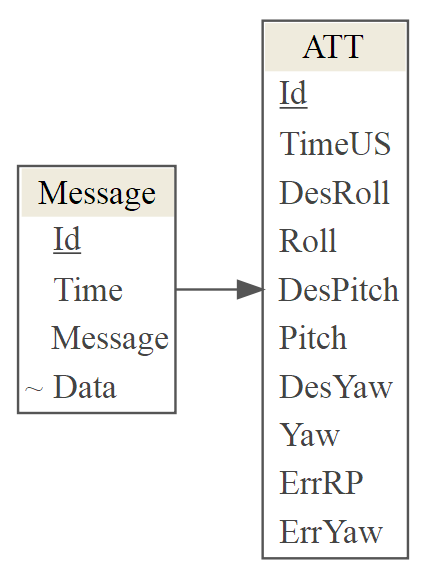
\includegraphics{./figure/1fn.PNG}
\caption{\label{fig:1fn}Message and ATT relationship.}
\end{figure}
Figure \ref{fig:1fn} has two tables where \emph{Message} table
represents all the different messages and table \emph{ATT} represents
any single \emph{data} table of a message - here the \emph{ATT} message.
From tables \ref{tab:att}, \ref{tab:rate} and \ref{tab:pidr} we can see
that the inner tables are of different shape. This means that each
message requires a separate table. The current \emph{Message} structure
does not permit more than one \emph{data} table to be used.

Another option would be to unwrap the inner \emph{data} table to be a
part of the outer \emph{Message} table. Here we run into a similar
problem. Since the inner \emph{data} tables are of different shape, the
single \emph{Message} table would have to contain each possible variable
in the logs and be empty most of the time. This table is realizable in a
database.
\begin{longtable}[]{@{}llllllllllll@{}}
\caption{\label{tab:message} \emph{Message} table.}\tabularnewline
\toprule
Id & Time & Message & TimeUS & DesRoll & Roll & .. & RDes & R & .. & Des
& P\tabularnewline
\midrule
\endfirsthead
\toprule
Id & Time & Message & TimeUS & DesRoll & Roll & .. & RDes & R & .. & Des
& P\tabularnewline
\midrule
\endhead
123 & time & ATT & value & value & value & .. & NA & NA & .. & NA &
NA\tabularnewline
124 & time & RATE & value & NA & NA & .. & value & value & .. & NA &
NA\tabularnewline
125 & time & PIDR & value & NA & NA & .. & NA & NA & .. & value &
value\tabularnewline
\bottomrule
\end{longtable}
This table contains mostly \emph{NA} values as for every message only a
subset of variables is relevant. When working with this table, the
\emph{NA} values need to be removed. We can solve this problem by
converting this table from wide form to long form. Since we are storing
several flights into the same database we need to add a flight
identificator.
\begin{longtable}[]{@{}lclllr@{}}
\caption{\label{tab:longtable} Long table.}\tabularnewline
\toprule
Id & Flight & Message & Timestamp & Parameter & Value\tabularnewline
\midrule
\endfirsthead
\toprule
Id & Flight & Message & Timestamp & Parameter & Value\tabularnewline
\midrule
\endhead
125 & 4 & ATT & 2018-03-23 17:26:57.12 & TimeUS &
2412496394\tabularnewline
126 & 4 & ATT & 2018-03-23 17:26:57.12 & DesRoll & -2.41\tabularnewline
127 & 4 & ATT & 2018-03-23 17:26:57.12 & Roll & -2.26\tabularnewline
\ldots{} & \ldots{} & \ldots{} & \ldots{} & \ldots{} &
\ldots{}\tabularnewline
134 & 4 & RATE & 2018-03-23 17:26:57.12 & TimeUS &
2412496408\tabularnewline
135 & 4 & RATE & 2018-03-23 17:26:57.12 & RDes &
-0.977470874786\tabularnewline
136 & 4 & RATE & 2018-03-23 17:26:57.12 & R &
0.30203345418\tabularnewline
\ldots{} & \ldots{} & \ldots{} & \ldots{} & \ldots{} &
\ldots{}\tabularnewline
145 & 4 & PIDR & 2018-03-23 17:26:57.12 & TimeUS &
2412496431\tabularnewline
146 & 4 & PIDR & 2018-03-23 17:26:57.12 & Des &
-0.0153276510537\tabularnewline
147 & 4 & PIDR & 2018-03-23 17:26:57.12 & P &
-0.00370784359984\tabularnewline
\bottomrule
\end{longtable}
In table \ref{tab:longtable} we added flight identificator but we would
like to have more information on the flights. To reduce metadata
repetition another table is needed. There is also quite a lot of
repetition in other values in the table. The message type and timestamp
repeat for each parameter in the inner table. The parameters also repeat
each time the message is repeated. Each of the repeating elements can be
moved to a dedicated table.
\begin{figure}
\centering
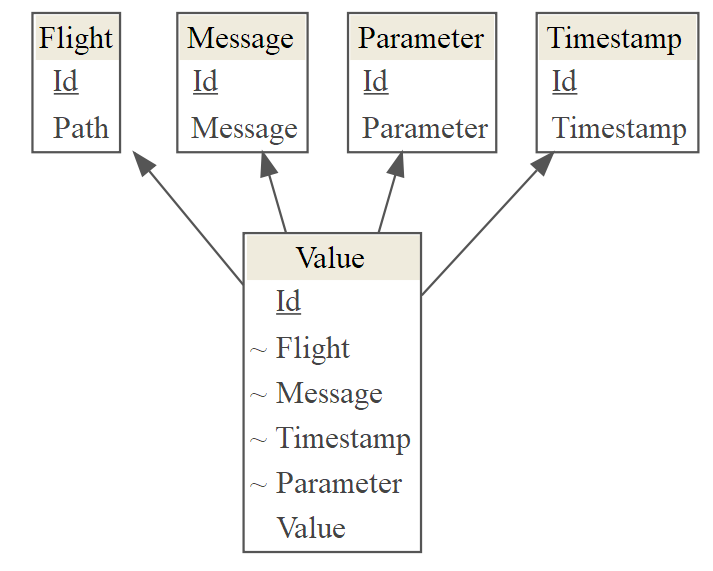
\includegraphics{./figure/databaseSchema.PNG}
\caption{\label{fig:database}Final database schema.}
\end{figure}
\section{The code}\label{the-code}

The code starts off with taking as an input the folder in which the
binary files is stored in. The folder is searched recursively so that
sub folders containing log files are also searched through. The files
are counted and the sizes saved. A filtering is done by file size. Files
larger than 100 MB and smaller than 4 MB are skipped. After the first
log file is processed the time taken is used to calculate an estimation
as to how long the whole process will take. Further more the total time
elapsed is also displayed.

\emph{Mavutil.py} from \emph{pymavlink} project is used for translating
the binary data to in memory representation. From there the data is
buffered and written to the \emph{SQLite} database. Each new message
type adds its parameter types to \emph{Parameter} table as seen in
figure \ref{fig:database} and each new message type is added to the
messages table. This allows for the specification for messages to change
and several versions of the specification to be used in different logs.
The message name and the parameter names are decoupled from each other.
An assumption that the message specification does not change in a single
log is made.

After processing a log a new entry to the \emph{Flight} table is made.
The metadata that is added is the path where the file was stored. As the
logs are separated into folders by which multirotor it was obtained from
or from which period in time or which version of the multirotor was used
then the path gives some sort of information that could be used for
filtering in the analysis stage.

Timestamps are allowed to repeat as searching through the whole table
means more processing needed while creating the database. This leaves a
possibility to create a secondary script that would look through the
\emph{Timestamp} table and removing duplicates and substituting the
\emph{Id} in the \emph{Value} table.

There is an overhead to writing into the \emph{SQLite} database. A
single write entails opening the database connection, writing to the
database and closing the connection. The opening and closing operation
adds an overhead that over hundreds of thousands of writes becomes
significant. To remedy this a bulk insert operation is available. Every
10 000 lines of the binary log a bulk write is done. That number is
experimental in nature as in testing making the number bigger did not
seem to save any processing time. Making it smaller however slows the
processing down. There is a possibility that further optimization can be
done.

In case where the script crashes or some error happens or new logs are
to be added to the database the code first checks the existence of the
database. If the database exists the supporting tables are read into
memory to be tested against so that new messages and parameters get
added to the database.

While \emph{SQLite} is a good option for an on disk storage of the
database, other databases are available and have some useful features.
One of which is the ability to use window functions on the database.
This means that it is possible to use filter kernels on the data while
still in database. Such functions using \emph{SQLite} require loading
the relevant segment of data (such as a single flight) into \emph{R}. An
attempt was made to port the working \emph{python} code to instead of
\emph{SQLite} to use \emph{PostgreSQL}\footnote{source (n.d.)}. The code
does work but is orders of magnitude slower. Heavy optimization is
needed to streamline the process and as \emph{SQLite} interface is
simpler in nature this idea was left as something to be done later given
more time. Moving to a full featured relational database management
system would allow easier porting of the analysis to a web based service
later, but that is not relevant in the context of this thesis.

The code for creating the database is written in \emph{python} and is
added to the appendix.

\chapter{Initial analysis of the
data}\label{initial-analysis-of-the-data}

As mentioned in the second chapter for the multirotor there is no
difference whether it is flying at a given direction at a set speed and
staying stationary in winds opposite to the flying direction of the
previous example and with the same speed as the multirotor was flying.
The following equation can be written:

\[\vec{w} = \vec{v} + \vec{u}\]

where \(\vec{w}\) is the ground speed of the multirotor, \(\vec{v}\) is
the wind speed of the multirotor and \(\vec{u}\) is the wind speed. If
we increase the wind speed \(\vec{u}\) the multirotor autopilot finds
the angles and motor power that allow it to fulfill the desired ground
speed \(\vec{w}\). When \(\vec{w}\) stays constant and \(\vec{u}\)
increases \(\vec{v}\) changes to account for the change in wind speed.
The change in \(\vec{v}\) is dependent on the flight direction and wind
direction. When flying against the wind \(\vec{w} = \vec{v} - \vec{u}\)
as the multirotor has to compensate for the increased wind speed. When
flying down wind the speeds add up - the multirotor has to do less work
to fly at the desired speed \(\vec{w}\). To find the wind speed a model
of the multirotor behavior is needed. Another way of looking at it is to
instead look for wind speed of the multirotor. This itself is the model
of the multirotor flight. The user gives the desired ground speed
\(\vec{w}\), the wind is \(\vec{u}\) and what we are after is the
resultant behavior \(\vec{v}\). To find the flight model \(\vec{v}\) we
can take the aforementioned equation and substitute the wind speed
\(\vec{u}\) with 0.

\[\vec{w} = \vec{v}\]

This way the desired speed equals the wind speed. With this in mind it
is necessary to extract from the database the data of the flights where
wind speed is close to zero to create the model. The chapter
\protect\hyperlink{extracting-windless-flight-data}{Extracting windless
flight data} does just that.

Another important factor to consider is the state of the battery. To
accurately model the multirotor behavior in diverse flight conditions
the information about how much energy is left is tantamount. In the
chapter \protect\hyperlink{analysis-of-battery-performance}{Analysis of
battery performance} the data available is analyzed.

\hypertarget{extracting-windless-flight-data}{\section{Extracting
windless flight data}\label{extracting-windless-flight-data}}

To find the flights where the wind is minimal we could look at the
levels of vibration aboard the multirotor but that is not the easiest
way nor is it very accurate due to its non-linear nature. Further more
the vibration levels stay relatively low for normal flight conditions.
As such it is more useful for estimating the upper limits of air speed
the multirotor is able to achieve.

A better option is to note that when wind speed is zero the multirotor
moves at the desired ground speed. If the desired ground speed is also
zero then the behavior of the multirotor should be stable as well.
Without wind the angles of the multirotor should fluctuate around zero
degrees and by looking at the average angles when the multirotor is
commanded to hold its position in \emph{loiter} or \emph{position}
\emph{hold} mode we can detect the logs that have nearly no wind. There
will be some fluctuation in the angles due to GPS inaccuracy and
barometric drift and drift of the IMU's and other sensors. This should
amount to white noise and average out given time. By taking the average
angles over the time of remaining stationary we will get the average
angle and direction of the wind as the multirotor will effectively be
flying to counteract the wind. Any sufficiently large angle constitutes
wind. For training the model only the windless flights are needed, but
since some wind is expected the level of cutoff where a flight is
considered to have been in windless condition. Various levels of
``windless'' data could be used as different cutoff values result in
different amounts of training data.
\begin{figure}
\centering
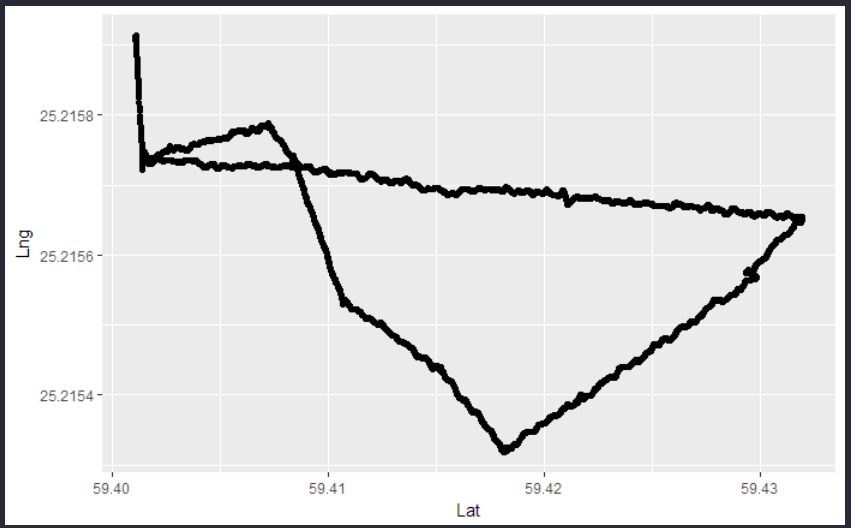
\includegraphics{./figure/latlng.PNG}
\caption{\label{fig:latlng}Latitude and longitude data points of a flight.}
\end{figure}
In figure \ref{fig:latlng} we can see a flight that consists of segments
of noisy data. This flight was mostly flown in manual \emph{loiter} mode
and as a result is this noisy.
\begin{figure}
\centering
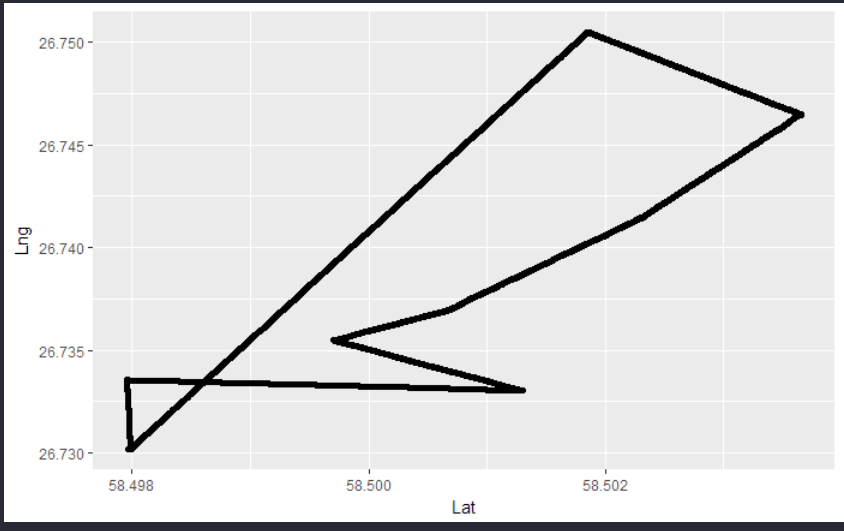
\includegraphics{./figure/latlng3.PNG}
\caption{\label{fig:latlngclean}Latitude and longitude data points of a
flight.}
\end{figure}
In figure \ref{fig:latlngclean} a flight using \emph{auto} mode is used.
In this mode the autopilot does its best to directly fly to the points
specified in the mission. While this information is useful for getting
an idea of the flight trajectory it does not help us with finding
windless flights as the information we are looking for is missing.
Namely the sections that the multirotor is stationary. Since the graph
does not contain any data about time, only individual points, we are
unable to see where the multirotor stands still. A guess would be that
at the turning points of the straight segments the multirotor could
potentially stand still.
\begin{figure}
\centering
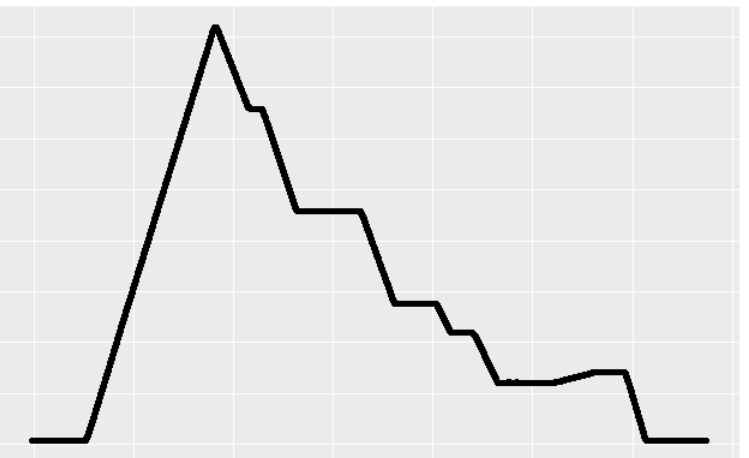
\includegraphics{./figure/lng.PNG}
\caption{\label{fig:lng}Longitude data points in timeseries of a flight.}
\end{figure}
Looking at the longitude time-series graph of the same flight on figure
\ref{fig:lng} we can clearly see where the multirotor stands still in
the longitude axis. However this is not sufficient to tell where the
multirotor is truly stationary as motion could be had on the latitude
axis.
\begin{figure}
\centering
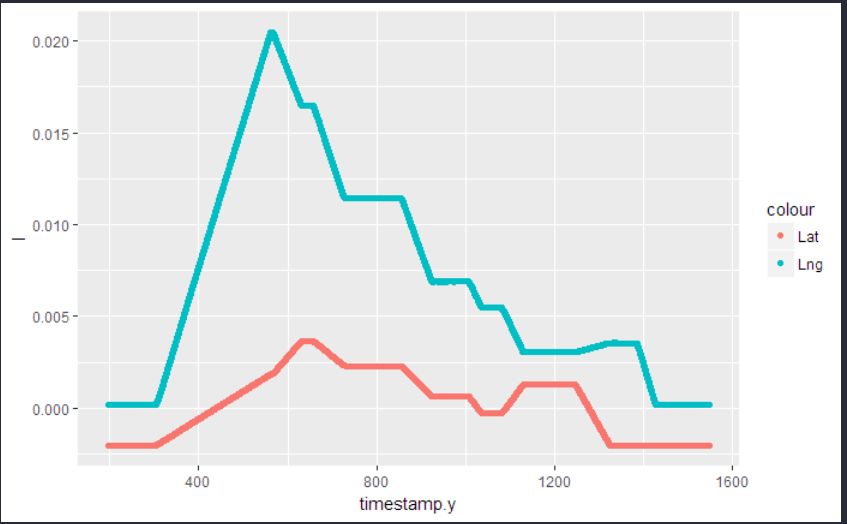
\includegraphics{./figure/latlngSamegraph.PNG}
\caption{\label{fig:lnglat}Longitude and latitude on the same timeseries
graph of a flight.}
\end{figure}
Figure \ref{fig:lnglat} has time on the x axis and latitude/longitude
point value changes on the y axis. The figure is made by taking both
latitude and longitude axes and merging them into a single one. Then the
data is shifted to very nearly zero so that both graphs can be seen.
This helps us see where the multirotor is actually stationary. Where the
value of both latitude and longitude stays unchanged for a period of
time the multirotor is stationary. Graphically we can see where this is
so but as a function of data we still need an additional function to
find the segments where the multirotor stays still. To find the segments
various approaches could be attempted. One of them would be to construct
lines through points in the time-series and looking for where the slope
of the line changes compared to the last one. Filtering would be needed
to account for the noise present. After that line segments where the
graph moves perpendicular to either latitude/longitude axis are taken
into consideration. From there latitude and longitude segments have to
be compared to find the segments where both are perpendicular to the
axis. This is to remove segments where motion is recorded as
perpendicular to either axis. This can be seen on the end of the
latitude longitude graphs on figure \ref{fig:lnglat}. There we can see
motion on the longitude graph but not on the latitude graph. Where both
graphs are parallel to time the multirotor is truly stationary. However
the aforementioned approach is not the best on as it ignores corner
cases such as when the multirotor has turned to face the direction of
future motion and taken some angle to start moving but from inertia has
not yet started moving. Luckily we have more parameters than latitude
and longitude coordinates in the logs. We also have information about
what mode the multirotor was in.
\begin{figure}
\centering
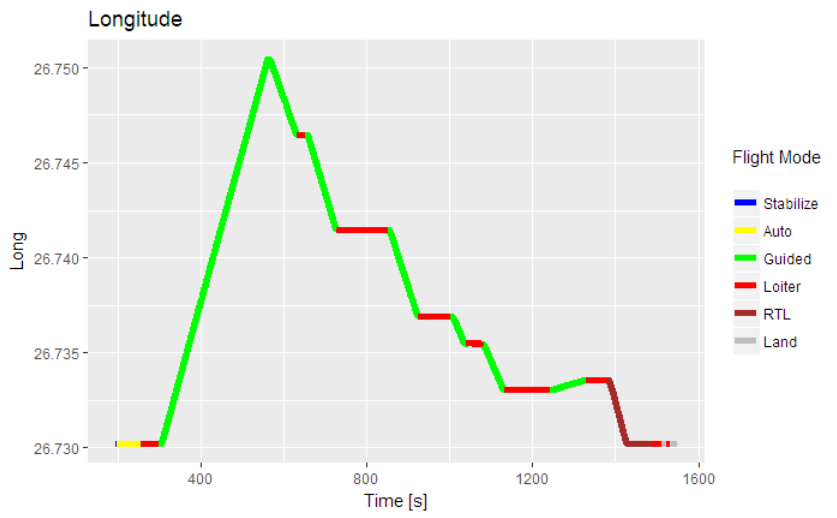
\includegraphics{./figure/longWithMode.PNG}
\caption{\label{fig:lngmode}Longitude data points in timeseries of a flight
augmented with mode information.}
\end{figure}
On figure \ref{fig:lngmode} the longitude time-series graph is augmented
with information about which mode the multirotor was in during the
flight. The take off sequence starts with brief entry to
\emph{stabilize} mode which we will ignore. After that \emph{auto} mode
with the setting to stay still until a non-empty mission is uploaded.
Soon after \emph{loiter} mode is entered. From figure \ref{fig:lnglat}
we can see that the multirotor remained stationary for the duration of
\emph{loiter} mode. After entering \emph{guided} mode, which is also an
automatic mission mode, the multirotor starts moving. In this flight
each time the multirotor is stationary the mode is \emph{loiter},
excepting take off sequence and landing procedure. In the landing
procedure the \emph{RTL} mode returns the multirotor to the launch
location and lands. During the landing the multirotor remains
stationary. Before fully landing the \emph{RTL} mode is interrupted by
the pilot by issuing \emph{loiter} command. We can assume that here we
had a skilled pilot who wanted to see how long the battery would last
until being truly empty and thus estimating the overall health of the
battery. After that an automatic landing fail-safe is executed by the
autopilot only to be interrupted again with the \emph{loiter} command by
the pilot. From this graph we can see that to find the windless flights
we need to find all flight segments where:
\begin{itemize}
\item
  The mode is \emph{loiter} and both latitude and longitude coordinates
  are stationary.
\item
  The segment after launch where the initial mission is empty and both
  latitude and longitude coordinates are stationary.
\end{itemize}
We could also use mode \emph{land} to check for wind conditions but it
needs to be taken into account that the latitude is changing and
\emph{land} and \emph{loiter} are not comparable. Also in \emph{land}
mode the multirotor can be manipulated manually so latitude and
longitude coordinates need to be checked for changes. \emph{RTL} mode
should be split in two parts since it internally contains both
\emph{guided} segment and \emph{land} segment. For the \emph{land} part
in \emph{RTL} same considerations need to be made.

Once the segments have been filtered out the average angle of the
multirotor needs to be calculated. Since the multirotor operates in
three dimensional space there are three angle parameters. As the vehicle
is capable of moving in any direction the orientation of the front is
not important for our purposes. The parameter for that is yaw. Instead
we average over the pitch and roll parameters.

The previous analysis is sufficient to filter help filter out relevant
flights from the database. From there the relevant data may be separated
into training and verification data to test the model. Further
decimation of data is needed as the data is collected at a high
frequency. The desired directions of flight need to be found from the
data as well as the desired flight speed. The exact details for the
model creation are left for the model creator.

After the model is created the direction of the wind needs to be
calculated. The direction of wind helps us optimize our battery use in
the case of automated missions. Flying against the wind takes more power
than flying by the wind. As we mentioned \(w = v + u\) which means that
the angle difference between \(w\) and \(u\) have to be compensated by
\(v\). Since all elements in the equation are vectors where the
magnitude is the speed of motion and the angle is the angle. By
subtracting from the desired ground speed \(w\) the model of the air
speed \(v\) we get the calculated wind speed \(u\). From here we can
extract the wind direction. The calculated wind speed can be compared to
real measurements to assess the accuracy of the model. An experiment may
be conducted by flying to multirotors with 10 to 100 meters apart from
each other where one of the multirotors is the multirotor from which the
model is built from. The other multirotor should carry an accurate wind
measurement device such as the one mentioned in \emph{Wind Estimation in
the Lower Atmosphere Using Multirotor Aircraft}\footnote{Palomaki et al.
  (2017)}. Both multirotors should fly at the same height and at the
same time to reduce variance of measurements in time. The missions
should be identical except for the spatial displacement to avoid
unwanted collisions.

\hypertarget{analysis-of-battery-performance}{\section{Analysis of
battery performance}\label{analysis-of-battery-performance}}
\begin{figure}
\centering
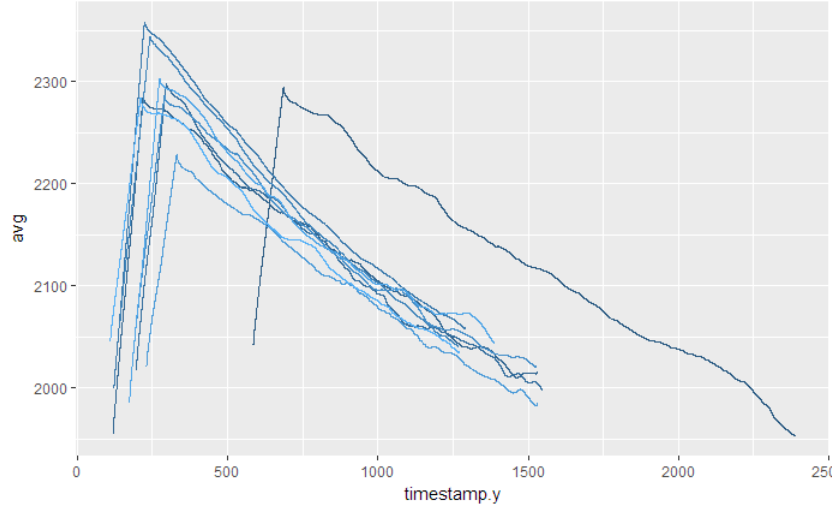
\includegraphics{./figure/akuGraafikutPekkis.PNG}
\caption{\label{fig:pekk}Low-pass filtered battery voltage graphs.}
\end{figure}
An figure \ref{fig:pekk} we have 9 heavily filtered graphs of voltage
during 9 flights. The smoothing is done by applying a moving average
filter with width of 1000 values to smooth the otherwise noisy graphs.
Here we can se a couple of problems. Firstly the beginnings are
distorted until the filter averages up to a more realistic value. These
parts need to be removed. Second problem is that since the logs start
before launch command the graphs can be shifted in time and thus not
align. This can be counter acted to shifting all the graphs by the first
voltage measurement value.
\begin{figure}
\centering
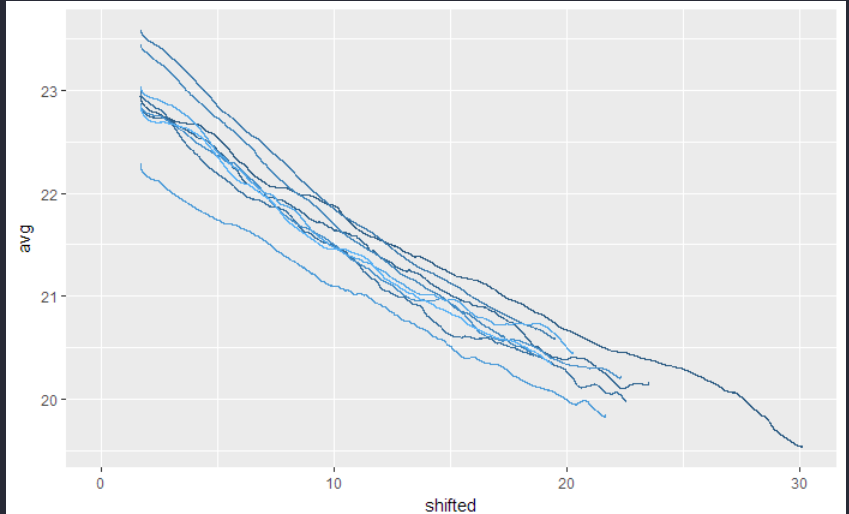
\includegraphics{./figure/akuGraafikudFixed.PNG}
\caption{\label{fig:fixed}Improved low-pass filtered battery voltage
graphs.}
\end{figure}
On figure \ref{fig:fixed} these problems have been rectified.
\begin{figure}
\centering
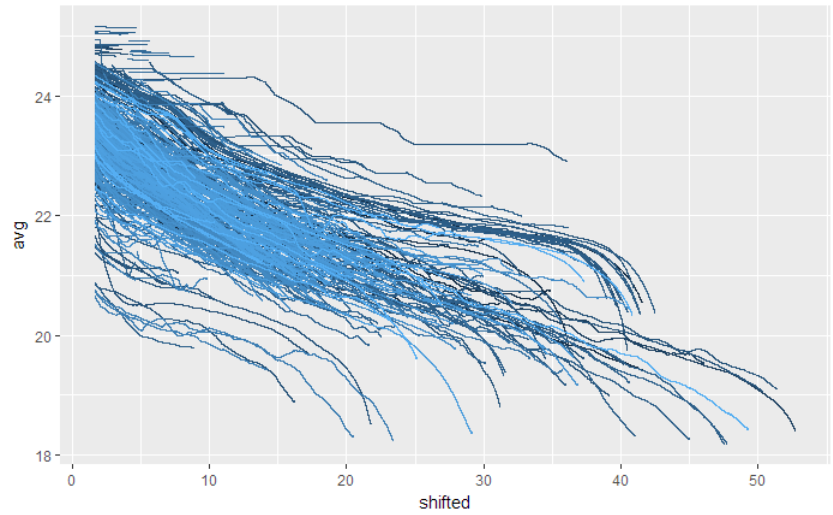
\includegraphics{./figure/allbat.PNG}
\caption{\label{fig:allbat}Improved low-pass filtered battery voltage graphs
of the whole database.}
\end{figure}
Figure \ref{fig:allbat} displays all the voltage graphs of all the
flights in the database. That is 1363 graphs. Here we can see that some
shorter flights are not really flights at all and need to be filtered
out from the database. We also see that there are at least two distinct
battery types used. Ones that fly for 40 minutes maintaining higher
voltage and ones that fly for longer while loosing voltage at a higher
rate. On the bottom left we can see a few graphs that start off by
dropping rapidly and then recovering a little. This is a sign of cold
batteries. The multirotor uses 550 watts on average and thus heats the
battery rapidly. Launching with a cold battery reduces the flight time
considerably but warming due to consumption helps restore some of the
capacity. This exemplifies the need for pre-heated batteries.
\begin{figure}
\centering
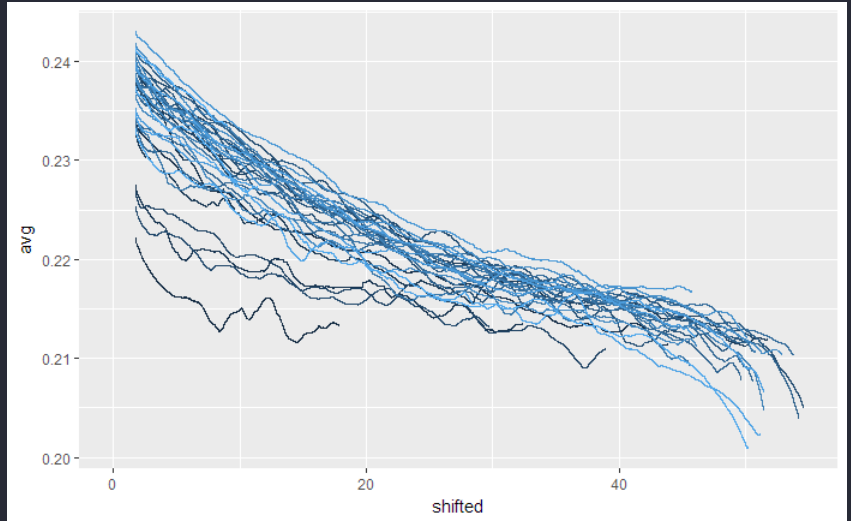
\includegraphics{./figure/rmkRohelineAku.PNG}
\caption{\label{fig:roheline}Improved low-pass filtered battery voltage
graphs of selected flights.}
\end{figure}
Figure \ref{fig:roheline} displays the graphs of a single multirotor
aircraft during a few days of time where counting wildlife in Estonian
woods was carried out. The graphs show the improved battery that is
capable of consistently flying for the guaranteed by Eli ltd 40 minutes
in good weather but also going above that and reaching 50 minutes on
most flights. On 4 graphs we can see the effects of not letting the
battery cool off after use and before recharging and not fully charging
the batteries.
\begin{figure}
\centering
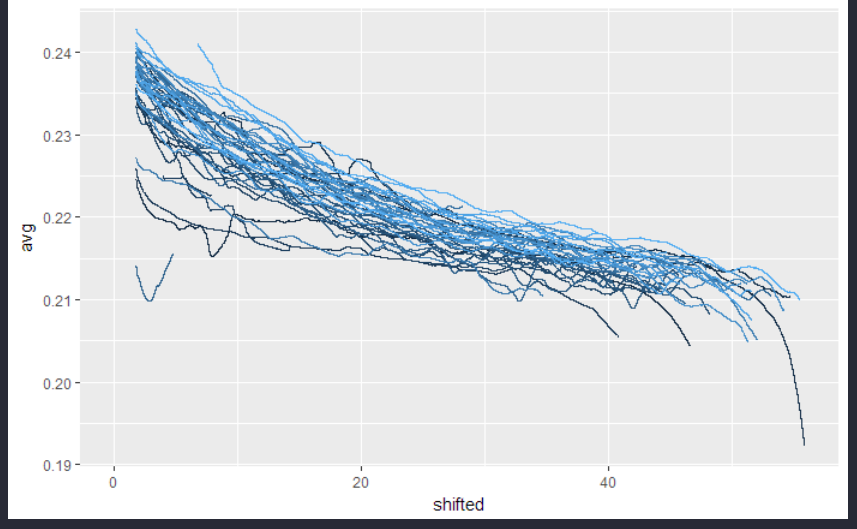
\includegraphics{./figure/rmkValgeAku.PNG}
\caption{\label{fig:valge}Improved low-pass filtered battery voltage graphs
of selected flights of another multirotor.}
\end{figure}
Figure \ref{fig:valge} displays the graphs of another multicopter that
was also used in the aforementioned missions. Here we can see that
during one flight the battery was allowed to empty more than usual. This
risks breaking the batteries.

From the graphs we can determine that battery estimation is very
difficult without knowing the type of the battery, the internal
temperature and the state of charge. Another important parameter is the
state of health of a battery as they degrade over time. Any smart
algorithm needs to take into account the wear and tear of the battery.
As long as there is no smart controller inside the battery to uniquely
identify it, give its state of charge and state of health any smart
algorithm will need to take into account the variability of the battery
output. A simplification can be made by expecting fully charged
batteries for every flight and placing that cognitive load on the pilot.
Each piece of missing information about the battery state requires a
bigger buffer for the safety mechanism reducing overall flight time and
distance.

\chapter*{Conclusion}\label{conclusion}
\addcontentsline{toc}{chapter}{Conclusion}

In order to create automatic missions that can be executed multiple
times without external input regardless of weather a model of the
multirotor behavior and a smart battery controller is needed. Until now
the main focus of research has been on improving the autopilot flight
controller algorithms.

Multiple data storage types were assessed. \emph{SQLite} was chosen to
be used as it is simple to use and acts like a real \emph{SQL} database
and it is easy to share as it is in a single file. Compared to other
options it takes less disk space.

The data representation was analyzed and designed for ease of use in the
analysis. The relevant code was created in \emph{python} programming
language converting the binary logs into \emph{SQLite} database. This
allows us to analyze several flights of data at the same time and make
comparisons. Until now the tools allowed for analysis of a single log at
a time. Further improvement suggestions were made.

Using the created database initial data analysis is done. As a result we
present the way to filter out the relevant data to train the model of
multirotor behavior on. Furthermore the need for a smart battery
controller is shown. An experiment to test the behavior model accuracy
in calculating wind speed and direction is proposed.

\appendix

\chapter{Python database creation
code}\label{python-database-creation-code}
\begin{Shaded}
\begin{Highlighting}[]
\CommentTok{#!c:\textbackslash{}python27\textbackslash{}python.exe}
\CommentTok{# -*- coding: utf-8 -*-}
\CommentTok{'''}
\CommentTok{read a mavlink binary file into SQLite database}
\CommentTok{'''}
\ImportTok{from}\NormalTok{ __future__ }\ImportTok{import}\NormalTok{ print_function}
\ImportTok{from}\NormalTok{ __future__ }\ImportTok{import}\NormalTok{ division}
\ImportTok{from}\NormalTok{ builtins   }\ImportTok{import} \BuiltInTok{range}
\ImportTok{from}\NormalTok{ argparse   }\ImportTok{import}\NormalTok{ ArgumentParser}
\ImportTok{from}\NormalTok{ pymavlink  }\ImportTok{import}\NormalTok{ mavutil}
\ImportTok{from}\NormalTok{ timeit     }\ImportTok{import}\NormalTok{ default_timer }\ImportTok{as}\NormalTok{ timer}
\ImportTok{import}\NormalTok{ os}
\ImportTok{import}\NormalTok{ sys}
\ImportTok{import}\NormalTok{ re}
\ImportTok{import}\NormalTok{ sqlite3}
\ImportTok{import}\NormalTok{ collections}
\ImportTok{import}\NormalTok{ datetime}
\ImportTok{import}\NormalTok{ math}
\NormalTok{extensions }\OperatorTok{=}\NormalTok{ collections.defaultdict(}\BuiltInTok{int}\NormalTok{)}
\KeywordTok{def}\NormalTok{ main(argv):}
    \CommentTok{# parser = ArgumentParser(description=__doc__)}
    \CommentTok{# parser.add_argument("database", help='Path to SQLite Database')}
    \CommentTok{# parser.add_argument("logs", metavar="LOG", nargs="+", }
      \CommentTok{# help='List of logs to process')}
    \CommentTok{# args = parser.parse_args(argv)}
    \CommentTok{# for filename in args.logs:}
    \CommentTok{#     process_tlog(filename)}
\NormalTok{    size }\OperatorTok{=} \DecValTok{0}
\NormalTok{    folder_path }\OperatorTok{=}\NormalTok{ argv[}\DecValTok{1}\NormalTok{]}
    \ControlFlowTok{for}\NormalTok{ path, dirs, files }\KeywordTok{in}\NormalTok{ os.walk(folder_path):}
        \ControlFlowTok{for}\NormalTok{ filename }\KeywordTok{in}\NormalTok{ files:}
            \ControlFlowTok{if}\NormalTok{ os.path.splitext(filename)[}\DecValTok{1}\NormalTok{].lower() }\OperatorTok{==} \StringTok{'.bin'}\NormalTok{:}
\NormalTok{                filesize }\OperatorTok{=}\NormalTok{ os.path.getsize(path}\OperatorTok{+}\NormalTok{os.sep}\OperatorTok{+}\NormalTok{filename)}
                \ControlFlowTok{if}\NormalTok{ filesize }\OperatorTok{<} \DecValTok{100000000} \KeywordTok{and}\NormalTok{ filesize }\OperatorTok{>} \DecValTok{4000000}\NormalTok{:}
\NormalTok{                    size }\OperatorTok{+=}\NormalTok{ filesize}
    \BuiltInTok{print}\NormalTok{(}\StringTok{'Total filesize to process: '} \OperatorTok{+}\NormalTok{ humanize_bytes(size))}
\NormalTok{    todo_size }\OperatorTok{=}\NormalTok{ size}
\NormalTok{    time_elapsed }\OperatorTok{=} \DecValTok{0}
    \ControlFlowTok{for}\NormalTok{ path, dirs, files }\KeywordTok{in}\NormalTok{ os.walk(folder_path):}
        \ControlFlowTok{for}\NormalTok{ filename }\KeywordTok{in}\NormalTok{ files:}
            \ControlFlowTok{if}\NormalTok{ os.path.splitext(filename)[}\DecValTok{1}\NormalTok{].lower() }\OperatorTok{==} \StringTok{'.bin'}\NormalTok{:}
\NormalTok{                filesize }\OperatorTok{=}\NormalTok{ os.path.getsize(path}\OperatorTok{+}\NormalTok{os.sep}\OperatorTok{+}\NormalTok{filename)}
                \ControlFlowTok{if}\NormalTok{ filesize }\OperatorTok{>} \DecValTok{100000000} \KeywordTok{or}\NormalTok{ filesize }\OperatorTok{<} \DecValTok{4000000}\NormalTok{:}
                    \ControlFlowTok{continue}
                \BuiltInTok{print}\NormalTok{(}\StringTok{'Processing file}\CharTok{\textbackslash{}t}\StringTok{File size}\CharTok{\textbackslash{}t}\StringTok{Folder'}\NormalTok{)}
                \BuiltInTok{print}\NormalTok{(}\StringTok{'}\SpecialCharTok{\{\}}\CharTok{\textbackslash{}t}\SpecialCharTok{\{\}}\CharTok{\textbackslash{}t\textbackslash{}t}\SpecialCharTok{\{\}}\StringTok{'}\NormalTok{.}\BuiltInTok{format}\NormalTok{(filename, }
\NormalTok{                  humanize_bytes(filesize), path))}
\NormalTok{                start }\OperatorTok{=}\NormalTok{ timer()}
\NormalTok{                process_tlog(path}\OperatorTok{+}\NormalTok{os.sep}\OperatorTok{+}\NormalTok{filename)    }
\NormalTok{                end }\OperatorTok{=}\NormalTok{ timer()}
\NormalTok{                diff }\OperatorTok{=}\NormalTok{ end}\OperatorTok{-}\NormalTok{start}
\NormalTok{                time_elapsed }\OperatorTok{+=}\NormalTok{ diff}
\NormalTok{                time_spent }\OperatorTok{=} \BuiltInTok{str}\NormalTok{(datetime.timedelta(}
\NormalTok{                  seconds}\OperatorTok{=}\NormalTok{math.floor(time_elapsed)))}
\NormalTok{                processing_time }\OperatorTok{=} \BuiltInTok{str}\NormalTok{(datetime.timedelta(}
\NormalTok{                  seconds}\OperatorTok{=}\NormalTok{math.floor(diff)))}
\NormalTok{                todo_size }\OperatorTok{-=}\NormalTok{ filesize}
\NormalTok{                processed }\OperatorTok{=}\NormalTok{ ((}\BuiltInTok{float}\NormalTok{(size) }\OperatorTok{-} \BuiltInTok{float}\NormalTok{(todo_size)) }\OperatorTok{/} 
                  \BuiltInTok{float}\NormalTok{(size)) }\OperatorTok{*} \BuiltInTok{float}\NormalTok{(}\DecValTok{100}\NormalTok{)}
\NormalTok{                bit_time }\OperatorTok{=} \BuiltInTok{float}\NormalTok{(diff) }\OperatorTok{/} \BuiltInTok{float}\NormalTok{(filesize)}
\NormalTok{                time_left }\OperatorTok{=} \BuiltInTok{str}\NormalTok{(datetime.timedelta(seconds}\OperatorTok{=}
\NormalTok{                  math.floor(}\BuiltInTok{float}\NormalTok{(bit_time) }\OperatorTok{*} \BuiltInTok{float}\NormalTok{(todo_size))))}
                \BuiltInTok{print}\NormalTok{(}\StringTok{"""File}\CharTok{\textbackslash{}t\textbackslash{}t}\StringTok{Processing Time}\CharTok{\textbackslash{}t}\StringTok{Time Elapsed}\CharTok{\textbackslash{}t}
\StringTok{                  Time Left}\CharTok{\textbackslash{}t}\StringTok{Percentage done"""}\NormalTok{)}
                \BuiltInTok{print}\NormalTok{(}\StringTok{'}\SpecialCharTok{\{\}}\CharTok{\textbackslash{}t}\SpecialCharTok{\{\}}\CharTok{\textbackslash{}t\textbackslash{}t}\SpecialCharTok{\{\}}\CharTok{\textbackslash{}t\textbackslash{}t}\SpecialCharTok{\{\}}\CharTok{\textbackslash{}t\textbackslash{}t}\SpecialCharTok{\{:2.2f\}}\StringTok{%'}\NormalTok{.}\BuiltInTok{format}\NormalTok{(filename, }
\NormalTok{                  processing_time, time_spent, time_left, processed))}
\KeywordTok{def}\NormalTok{ process_tlog(filename):}
    \CommentTok{'''convert a ardupilot BIN file to SQLite database'''}
\NormalTok{    mlog }\OperatorTok{=}\NormalTok{ mavutil.mavlink_connection(filename, dialect}\OperatorTok{=}\StringTok{'ardupilotmega'}\NormalTok{, }
\NormalTok{      zero_time_base}\OperatorTok{=}\VariableTok{True}\NormalTok{)}
\NormalTok{    connection }\OperatorTok{=}\NormalTok{ create_connection(}\StringTok{'rmkRoheline.db'}\NormalTok{)}
    \CommentTok{# conn = create_connection(args.database)}
\NormalTok{    database }\OperatorTok{=}\NormalTok{ \{\}}
    \ControlFlowTok{try}\NormalTok{:}
\NormalTok{        database }\OperatorTok{=}\NormalTok{ load_database_to_ram(connection)}
    \ControlFlowTok{except}\NormalTok{:}
\NormalTok{        database }\OperatorTok{=}\NormalTok{ create_database(connection)}
\NormalTok{    add_flight(database, filename, connection)}
\NormalTok{    counter }\OperatorTok{=} \DecValTok{0}
    \ControlFlowTok{while} \VariableTok{True}\NormalTok{:}
\NormalTok{        line }\OperatorTok{=}\NormalTok{ mlog.recv_match()}
        \CommentTok{# Exit on file end}
        \ControlFlowTok{if}\NormalTok{ line }\KeywordTok{is} \VariableTok{None}\NormalTok{:}
            \ControlFlowTok{break}
\NormalTok{        message }\OperatorTok{=}\NormalTok{ line.get_type()}
        \CommentTok{# Remove bad packets}
        \ControlFlowTok{if}\NormalTok{ message }\OperatorTok{==} \StringTok{'BAD_DATA'}\NormalTok{:}
            \ControlFlowTok{continue}
        \CommentTok{# FMT defines the format and PARM is params... }
        \CommentTok{# not sure if i need em or not}
        \ControlFlowTok{if}\NormalTok{ message }\KeywordTok{in}\NormalTok{ [}\StringTok{'FMT'}\NormalTok{, }\StringTok{'PARM'}\NormalTok{]:}
            \ControlFlowTok{continue}
\NormalTok{        process_header(line, database, connection)}
\NormalTok{        process_data(line, database)}
\NormalTok{        counter}\OperatorTok{+=}\DecValTok{1}
        \ControlFlowTok{if}\NormalTok{ counter }\OperatorTok{%} \DecValTok{10000} \OperatorTok{==} \DecValTok{0}\NormalTok{:}
\NormalTok{            bulk_write_values(database, connection)}
\NormalTok{            bulk_write_timestamps(database, connection)}
\NormalTok{    bulk_write_values(database, connection)}
\NormalTok{    bulk_write_timestamps(database, connection)}
\NormalTok{    connection.commit()}
\NormalTok{    connection.close()}
\KeywordTok{def}\NormalTok{ process_header(line, database, connection):}
\NormalTok{    message }\OperatorTok{=}\NormalTok{ line.get_type()}
    \ControlFlowTok{if}\NormalTok{ message }\KeywordTok{not} \KeywordTok{in}\NormalTok{ database[}\StringTok{'messages'}\NormalTok{]:}
\NormalTok{        add_message(message, database, connection)}
\NormalTok{    fieldnames }\OperatorTok{=}\NormalTok{ line._fieldnames}
\NormalTok{    parameters }\OperatorTok{=}\NormalTok{ []}
    \ControlFlowTok{for}\NormalTok{ field }\KeywordTok{in}\NormalTok{ fieldnames:}
\NormalTok{        val }\OperatorTok{=} \BuiltInTok{getattr}\NormalTok{(line, field)}
        \ControlFlowTok{if} \KeywordTok{not} \BuiltInTok{isinstance}\NormalTok{(val, }\BuiltInTok{str}\NormalTok{):}
            \ControlFlowTok{if} \BuiltInTok{type}\NormalTok{(val) }\KeywordTok{is} \KeywordTok{not} \BuiltInTok{list}\NormalTok{:}
\NormalTok{                parameters.append(field)}
            \ControlFlowTok{else}\NormalTok{:}
                \ControlFlowTok{for}\NormalTok{ i }\KeywordTok{in} \BuiltInTok{range}\NormalTok{(}\DecValTok{0}\NormalTok{, }\BuiltInTok{len}\NormalTok{(val)):}
\NormalTok{                    parameters.append(field }\OperatorTok{+} \StringTok{'}\SpecialCharTok\NormalTok{ i}\OperatorTok{+}\DecValTok{1}\NormalTok{) }
    
\NormalTok{    add_parameters(parameters, database, connection)}
    \ControlFlowTok{if} \StringTok{'buffer'} \KeywordTok{not} \KeywordTok{in}\NormalTok{ database:}
\NormalTok{        database[}\StringTok{'buffer'}\NormalTok{] }\OperatorTok{=}\NormalTok{ \{\}}
\NormalTok{    database[}\StringTok{'buffer'}\NormalTok{][message] }\OperatorTok{=}\NormalTok{ parameters}
\KeywordTok{def}\NormalTok{ process_data(line, database):        }
    \CommentTok{# add message type with parameters to buffer to be able }
    \CommentTok{# to save to sqlite db later}
\NormalTok{    message }\OperatorTok{=}\NormalTok{ line.get_type()}
\NormalTok{    fieldnames }\OperatorTok{=}\NormalTok{ line._fieldnames}
\NormalTok{    data }\OperatorTok{=}\NormalTok{ []}
\NormalTok{    add_timestamp(line._timestamp, database)}
    \ControlFlowTok{for}\NormalTok{ field }\KeywordTok{in}\NormalTok{ fieldnames:}
\NormalTok{        val }\OperatorTok{=} \BuiltInTok{getattr}\NormalTok{(line, field)}
        \ControlFlowTok{if} \KeywordTok{not} \BuiltInTok{isinstance}\NormalTok{(val, }\BuiltInTok{str}\NormalTok{):}
            \ControlFlowTok{if} \BuiltInTok{type}\NormalTok{(val) }\KeywordTok{is} \KeywordTok{not} \BuiltInTok{list}\NormalTok{:}
\NormalTok{                data.append(}\StringTok{"}\SpecialCharTok\NormalTok{ val)}
            \ControlFlowTok{else}\NormalTok{:}
                \ControlFlowTok{for}\NormalTok{ i }\KeywordTok{in} \BuiltInTok{range}\NormalTok{(}\DecValTok{0}\NormalTok{, }\BuiltInTok{len}\NormalTok{(val)):}
\NormalTok{                    data.append(}\StringTok{"}\SpecialCharTok\NormalTok{ val[i])}
    
\NormalTok{    parameters_and_values }\OperatorTok{=} \BuiltInTok{zip}\NormalTok{(database[}\StringTok{'buffer'}\NormalTok{][message], data)}
\NormalTok{    parameter }\OperatorTok{=} \DecValTok{0}
\NormalTok{    value }\OperatorTok{=} \DecValTok{1}
    \ControlFlowTok{if} \StringTok{'values'} \KeywordTok{not} \KeywordTok{in}\NormalTok{ database[}\StringTok{'buffer'}\NormalTok{]:}
\NormalTok{        database[}\StringTok{'buffer'}\NormalTok{][}\StringTok{'values'}\NormalTok{] }\OperatorTok{=}\NormalTok{ []}
    \ControlFlowTok{for}\NormalTok{ parameter_pair }\KeywordTok{in}\NormalTok{ parameters_and_values:}
\NormalTok{        database[}\StringTok{'last value id'}\NormalTok{] }\OperatorTok{+=} \DecValTok{1}
\NormalTok{        database[}\StringTok{'buffer'}\NormalTok{][}\StringTok{'values'}\NormalTok{].append((}
\NormalTok{            database[}\StringTok{'last value id'}\NormalTok{],}
\NormalTok{            database[}\StringTok{'last flight id'}\NormalTok{],}
\NormalTok{            database[}\StringTok{'last timestamp id'}\NormalTok{],}
\NormalTok{            database[}\StringTok{'messages'}\NormalTok{][message],}
\NormalTok{            database[}\StringTok{'parameters'}\NormalTok{][parameter_pair[parameter]],}
\NormalTok{            parameter_pair[value]}
\NormalTok{        ))}
\KeywordTok{def}\NormalTok{ load_database_to_ram(connection):    }
    \CommentTok{""" load a database specified by connection into memory}
\CommentTok{    :param connection: connection to database}
\CommentTok{    :return: database}
\CommentTok{    """}
\NormalTok{    cursor }\OperatorTok{=}\NormalTok{ connection.cursor()}
\NormalTok{    cursor.execute(}\StringTok{'SELECT * FROM parameter'}\NormalTok{)}
\NormalTok{    parameters }\OperatorTok{=} \BuiltInTok{dict}\NormalTok{(}\BuiltInTok{map}\NormalTok{(}\KeywordTok{lambda}\NormalTok{ (}\BuiltInTok{id}\NormalTok{, name): (name.encode(}\StringTok{'ascii'}\NormalTok{), }
      \BuiltInTok{id}\NormalTok{), cursor.fetchall()))}
\NormalTok{    cursor.execute(}\StringTok{'SELECT * FROM message'}\NormalTok{)}
\NormalTok{    messages }\OperatorTok{=} \BuiltInTok{dict}\NormalTok{(}\BuiltInTok{map}\NormalTok{(}\KeywordTok{lambda}\NormalTok{ (}\BuiltInTok{id}\NormalTok{, name): (name.encode(}\StringTok{'ascii'}\NormalTok{), }
      \BuiltInTok{id}\NormalTok{), cursor.fetchall()))}
\NormalTok{    cursor.execute(}\StringTok{'SELECT * FROM parameter ORDER BY id DESC LIMIT 1'}\NormalTok{)}
\NormalTok{    last_parameter_id }\OperatorTok{=}\NormalTok{ (cursor.fetchall())[}\DecValTok{0}\NormalTok{][}\DecValTok{0}\NormalTok{]}
\NormalTok{    cursor.execute(}\StringTok{'SELECT * FROM message ORDER BY id DESC LIMIT 1'}\NormalTok{)}
\NormalTok{    last_message_id }\OperatorTok{=}\NormalTok{ (cursor.fetchall())[}\DecValTok{0}\NormalTok{][}\DecValTok{0}\NormalTok{]}
\NormalTok{    cursor.execute(}\StringTok{'SELECT * FROM timestamp ORDER BY id DESC LIMIT 1'}\NormalTok{)}
\NormalTok{    last_timestamp_id }\OperatorTok{=}\NormalTok{ (cursor.fetchall())[}\DecValTok{0}\NormalTok{][}\DecValTok{0}\NormalTok{]}
\NormalTok{    cursor.execute(}\StringTok{'SELECT * FROM value ORDER BY id DESC LIMIT 1'}\NormalTok{)}
\NormalTok{    last_value_id }\OperatorTok{=}\NormalTok{ (cursor.fetchall())[}\DecValTok{0}\NormalTok{][}\DecValTok{0}\NormalTok{]}
\NormalTok{    cursor.execute(}\StringTok{'SELECT * FROM flight ORDER BY id DESC LIMIT 1'}\NormalTok{)}
\NormalTok{    last_flight_id }\OperatorTok{=}\NormalTok{ (cursor.fetchall())[}\DecValTok{0}\NormalTok{][}\DecValTok{0}\NormalTok{]}
\NormalTok{    database }\OperatorTok{=}\NormalTok{ \{}
        \StringTok{'last value id'}\NormalTok{: last_value_id,}
        \StringTok{'last flight id'}\NormalTok{: last_flight_id,}
        \StringTok{'last message id'}\NormalTok{: last_message_id,}
        \StringTok{'last timestamp id'}\NormalTok{: last_timestamp_id,}
        \StringTok{'last parameter id'}\NormalTok{: last_parameter_id,}
        \StringTok{'messages'}\NormalTok{: messages,}
        \StringTok{'parameters'}\NormalTok{: parameters}
\NormalTok{    \}}
    \ControlFlowTok{return}\NormalTok{ database}
\KeywordTok{def}\NormalTok{ create_database(connection):    }
    \CommentTok{""" create a database specified by connection and leave a copy }
\CommentTok{    into memory}
\CommentTok{    :param connection: connection to database}
\CommentTok{    :return: database}
\CommentTok{    """}
\NormalTok{    cursor }\OperatorTok{=}\NormalTok{ connection.cursor()}
\NormalTok{    cursor.execute(}\StringTok{"""}
\StringTok{      CREATE TABLE flight (}
\StringTok{        id INTEGER NOT NULL PRIMARY KEY, }
\StringTok{        path TEXT}
\StringTok{        )}
\StringTok{      """}\NormalTok{)}
\NormalTok{    cursor.execute(}\StringTok{"""}
\StringTok{      CREATE TABLE message (}
\StringTok{        id INTEGER NOT NULL PRIMARY KEY, }
\StringTok{        message TEXT}
\StringTok{        )}
\StringTok{      """}\NormalTok{)}
\NormalTok{    cursor.execute(}\StringTok{"""}
\StringTok{      CREATE TABLE timestamp (}
\StringTok{        id INTEGER NOT NULL PRIMARY KEY, }
\StringTok{        timestamp INTEGER}
\StringTok{        )}
\StringTok{      """}\NormalTok{)}
\NormalTok{    cursor.execute(}\StringTok{"""}
\StringTok{      CREATE TABLE parameter (}
\StringTok{        id INTEGER NOT NULL PRIMARY KEY, }
\StringTok{        parameter TEXT}
\StringTok{        )}
\StringTok{      """}\NormalTok{)}
\NormalTok{    cursor.execute(}\StringTok{"""}
\StringTok{    CREATE TABLE value (}
\StringTok{        id INTEGER NOT NULL PRIMARY KEY,}
\StringTok{        flight INTEGER NOT NULL,}
\StringTok{        message INTEGER NOT NULL,}
\StringTok{        timestamp INTEGER NOT NULL,}
\StringTok{        parameter INTEGER NOT NULL,}
\StringTok{        value REAL,}
\StringTok{        FOREIGN KEY(flight) REFERENCES flight(id)}
\StringTok{        FOREIGN KEY(message) REFERENCES message(id)}
\StringTok{        FOREIGN KEY(timestamp) REFERENCES timestamp(id)}
\StringTok{        FOREIGN KEY(parameter) REFERENCES parameter(id)}
\StringTok{    )"""}\NormalTok{)}
\NormalTok{    database }\OperatorTok{=}\NormalTok{ \{}
        \StringTok{'last flight id'}\NormalTok{: }\DecValTok{0}\NormalTok{,}
        \StringTok{'last message id'}\NormalTok{: }\DecValTok{0}\NormalTok{,}
        \StringTok{'last timestamp id'}\NormalTok{: }\DecValTok{0}\NormalTok{,}
        \StringTok{'last parameter id'}\NormalTok{: }\DecValTok{0}\NormalTok{,}
        \StringTok{'last value id'}\NormalTok{: }\DecValTok{0}\NormalTok{,}
        \StringTok{'messages'}\NormalTok{: \{\},}
        \StringTok{'parameters'}\NormalTok{: \{\}}
\NormalTok{    \}}
    \ControlFlowTok{return}\NormalTok{ database}
\KeywordTok{def}\NormalTok{ bulk_write_values(database, connection):}
    \CommentTok{# write buffered values to database}
\NormalTok{    cursor }\OperatorTok{=}\NormalTok{ connection.cursor()}
\NormalTok{    sql }\OperatorTok{=}\NormalTok{ get_sql(}\StringTok{'value'}\NormalTok{,[}\StringTok{'id'}\NormalTok{, }\StringTok{'flight'}\NormalTok{, }\StringTok{'timestamp'}\NormalTok{, }\StringTok{'message'}\NormalTok{, }
      \StringTok{'parameter'}\NormalTok{, }\StringTok{'value'}\NormalTok{])}
\NormalTok{    cursor.executemany(sql, database[}\StringTok{'buffer'}\NormalTok{][}\StringTok{'values'}\NormalTok{])}
\NormalTok{    database[}\StringTok{'buffer'}\NormalTok{][}\StringTok{'values'}\NormalTok{] }\OperatorTok{=}\NormalTok{ []}
\KeywordTok{def}\NormalTok{ bulk_write_timestamps(database, connection):}
\NormalTok{    cursor }\OperatorTok{=}\NormalTok{ connection.cursor()}
\NormalTok{    sql }\OperatorTok{=}\NormalTok{ get_sql(}\StringTok{'timestamp'}\NormalTok{,[}\StringTok{'id'}\NormalTok{, }\StringTok{'timestamp'}\NormalTok{])}
\NormalTok{    cursor.executemany(sql, database[}\StringTok{'buffer'}\NormalTok{][}\StringTok{'timestamps'}\NormalTok{])}
\NormalTok{    database[}\StringTok{'buffer'}\NormalTok{][}\StringTok{'timestamps'}\NormalTok{] }\OperatorTok{=}\NormalTok{ []}
\KeywordTok{def}\NormalTok{ add_flight(database, filename, connection):}
\NormalTok{    database[}\StringTok{'last flight id'}\NormalTok{] }\OperatorTok{+=} \DecValTok{1}    
\NormalTok{    cursor }\OperatorTok{=}\NormalTok{ connection.cursor()}
\NormalTok{    sql }\OperatorTok{=} \StringTok{'INSERT INTO flight(id, path) VALUES(?,?)'}
\NormalTok{    cursor.execute(sql, [database[}\StringTok{'last flight id'}\NormalTok{], scrub(filename)])}
\KeywordTok{def}\NormalTok{ add_message(message, database, connection):}
\NormalTok{    database[}\StringTok{'last message id'}\NormalTok{] }\OperatorTok{+=} \DecValTok{1}
\NormalTok{    database[}\StringTok{'messages'}\NormalTok{][message] }\OperatorTok{=}\NormalTok{ database[}\StringTok{'last message id'}\NormalTok{]}
\NormalTok{    sql }\OperatorTok{=}\NormalTok{ get_sql(}\StringTok{'message'}\NormalTok{, [}\StringTok{'id'}\NormalTok{, }\StringTok{'message'}\NormalTok{])}
\NormalTok{    data }\OperatorTok{=}\NormalTok{ (database[}\StringTok{'messages'}\NormalTok{][message], message)}
\NormalTok{    cursor }\OperatorTok{=}\NormalTok{ connection.cursor()}
\NormalTok{    cursor.execute(sql, data)}
\KeywordTok{def}\NormalTok{ add_timestamp(timestamp, database):}
    \ControlFlowTok{if} \StringTok{'timestamps'} \KeywordTok{not} \KeywordTok{in}\NormalTok{ database[}\StringTok{'buffer'}\NormalTok{]:}
\NormalTok{        database[}\StringTok{'buffer'}\NormalTok{][}\StringTok{'timestamps'}\NormalTok{] }\OperatorTok{=}\NormalTok{ []}
\NormalTok{    database[}\StringTok{'last timestamp id'}\NormalTok{] }\OperatorTok{+=} \DecValTok{1}
\NormalTok{    database[}\StringTok{'buffer'}\NormalTok{][}\StringTok{'timestamps'}\NormalTok{].append((}
\NormalTok{      database[}\StringTok{'last timestamp id'}\NormalTok{], timestamp))}
\KeywordTok{def}\NormalTok{ add_parameters(parameters, database, connection):}
    \BuiltInTok{buffer} \OperatorTok{=}\NormalTok{ []}
\NormalTok{    params }\OperatorTok{=} \BuiltInTok{filter}\NormalTok{(}\KeywordTok{lambda}\NormalTok{ p: p }\KeywordTok{not} \KeywordTok{in} 
\NormalTok{      database[}\StringTok{'parameters'}\NormalTok{], parameters)}
    \ControlFlowTok{for}\NormalTok{ parameter }\KeywordTok{in}\NormalTok{ params:}
\NormalTok{        database[}\StringTok{'last parameter id'}\NormalTok{] }\OperatorTok{+=} \DecValTok{1}
\NormalTok{        database[}\StringTok{'parameters'}\NormalTok{][parameter] }\OperatorTok{=}\NormalTok{ database[}\StringTok{'last parameter id'}\NormalTok{]}
        \BuiltInTok{buffer}\NormalTok{.append((database[}\StringTok{'last parameter id'}\NormalTok{], parameter))}
    
\NormalTok{    sql }\OperatorTok{=}\NormalTok{ get_sql(}\StringTok{'parameter'}\NormalTok{, [}\StringTok{'id'}\NormalTok{, }\StringTok{'parameter'}\NormalTok{])}
\NormalTok{    cursor }\OperatorTok{=}\NormalTok{ connection.cursor()}
\NormalTok{    cursor.executemany(sql, }\BuiltInTok{buffer}\NormalTok{)}
\NormalTok{    connection.commit()}
\KeywordTok{def}\NormalTok{ get_sql(table_name, column_names):}
\NormalTok{    questionmarks }\OperatorTok{=} \StringTok{','}\NormalTok{.join(}\BuiltInTok{map}\NormalTok{(}\KeywordTok{lambda}\NormalTok{ x: }\StringTok{'?'}\NormalTok{, column_names))}
\NormalTok{    column_names_string }\OperatorTok{=} \StringTok{','}\NormalTok{.join(column_names)}
    \ControlFlowTok{return} \StringTok{'INSERT INTO }\SpecialCharTok{\{\}}\StringTok{(}\SpecialCharTok{\{\}}\StringTok{) VALUES(}\SpecialCharTok{\{\}}\StringTok{)'}\NormalTok{.}\BuiltInTok{format}\NormalTok{(scrub(table_name), }
\NormalTok{      column_names_string, questionmarks)}
\KeywordTok{def}\NormalTok{ create_connection(db_file):}
    \CommentTok{""" create a database connection to the SQLite database}
\CommentTok{        specified by db_file}
\CommentTok{    :param db_file: database file}
\CommentTok{    :return: Connection object or None}
\CommentTok{    """}
    \ControlFlowTok{try}\NormalTok{:}
\NormalTok{        conn }\OperatorTok{=}\NormalTok{ sqlite3.}\ExtensionTok{connect}\NormalTok{(db_file)}
        \ControlFlowTok{return}\NormalTok{ conn}
    \ControlFlowTok{except} \PreprocessorTok{Exception} \ImportTok{as}\NormalTok{ e:}
        \BuiltInTok{print}\NormalTok{(e)}
    \ControlFlowTok{return} \VariableTok{None}
\KeywordTok{def}\NormalTok{ scrub(table_name):}
    \ControlFlowTok{return} \StringTok{''}\NormalTok{.join( }\BuiltInTok{chr} \ControlFlowTok{for} \BuiltInTok{chr} \KeywordTok{in}\NormalTok{ table_name }\ControlFlowTok{if} \BuiltInTok{chr}\NormalTok{.isalnum())}
\KeywordTok{def}\NormalTok{ humanize_bytes(}\BuiltInTok{bytes}\NormalTok{, precision}\OperatorTok{=}\DecValTok{1}\NormalTok{):}
    \CommentTok{"""Return a humanized string representation of a number of bytes.}
\CommentTok{    Assumes `from __future__ import division`.}
\CommentTok{    >>> humanize_bytes(1)}
\CommentTok{    '1 byte'}
\CommentTok{    >>> humanize_bytes(1024)}
\CommentTok{    '1.0 kB'}
\CommentTok{    >>> humanize_bytes(1024*123)}
\CommentTok{    '123.0 kB'}
\CommentTok{    >>> humanize_bytes(1024*12342)}
\CommentTok{    '12.1 MB'}
\CommentTok{    >>> humanize_bytes(1024*12342,2)}
\CommentTok{    '12.05 MB'}
\CommentTok{    >>> humanize_bytes(1024*1234,2)}
\CommentTok{    '1.21 MB'}
\CommentTok{    >>> humanize_bytes(1024*1234*1111,2)}
\CommentTok{    '1.31 GB'}
\CommentTok{    >>> humanize_bytes(1024*1234*1111,1)}
\CommentTok{    '1.3 GB'}
\CommentTok{    """}
\NormalTok{    abbrevs }\OperatorTok{=}\NormalTok{ (}
\NormalTok{        (}\DecValTok{1}\OperatorTok{<<}\NormalTok{50L, }\StringTok{'PB'}\NormalTok{),}
\NormalTok{        (}\DecValTok{1}\OperatorTok{<<}\NormalTok{40L, }\StringTok{'TB'}\NormalTok{),}
\NormalTok{        (}\DecValTok{1}\OperatorTok{<<}\NormalTok{30L, }\StringTok{'GB'}\NormalTok{),}
\NormalTok{        (}\DecValTok{1}\OperatorTok{<<}\NormalTok{20L, }\StringTok{'MB'}\NormalTok{),}
\NormalTok{        (}\DecValTok{1}\OperatorTok{<<}\NormalTok{10L, }\StringTok{'kB'}\NormalTok{),}
\NormalTok{        (}\DecValTok{1}\NormalTok{, }\StringTok{'bytes'}\NormalTok{)}
\NormalTok{    )}
    \ControlFlowTok{if} \BuiltInTok{bytes} \OperatorTok{==} \DecValTok{1}\NormalTok{:}
        \ControlFlowTok{return} \StringTok{'1 byte'}
    \ControlFlowTok{for}\NormalTok{ factor, suffix }\KeywordTok{in}\NormalTok{ abbrevs:}
        \ControlFlowTok{if} \BuiltInTok{bytes} \OperatorTok{>=}\NormalTok{ factor:}
            \ControlFlowTok{break}
    \ControlFlowTok{return} \StringTok{'}\SpecialCharTok{%.*f}\StringTok{ }\SpecialCharTok\NormalTok{ (precision, }\BuiltInTok{bytes} \OperatorTok{/}\NormalTok{ factor, suffix)}
\ControlFlowTok{if} \VariableTok{__name__} \OperatorTok{==} \StringTok{"__main__"}\NormalTok{:}
\NormalTok{     main(sys.argv)}
\end{Highlighting}
\end{Shaded}
\backmatter

\chapter*{References}\label{references}
\addcontentsline{toc}{chapter}{References}

\markboth{References}{References}

\noindent

\setlength{\parindent}{-0.20in} \setlength{\leftskip}{0.20in}
\setlength{\parskip}{8pt}

\hypertarget{refs}{}
\hypertarget{ref-sqlite}{}
About sqlite. (n.d.). \emph{SQLite Home Page}. Retrieved from
\url{https://www.sqlite.org/about.html}

\hypertarget{ref-rjon}{}
Couture-Beil, A. (2014). \emph{Rjson: JSON for r}. Retrieved from
\url{https://CRAN.R-project.org/package=rjson}

\hypertarget{ref-json}{}
Crockford, D. (n.d.). JavaScript object notation. \emph{JSON}. Retrieved
from \url{https://WWW.json.org/}

\hypertarget{ref-codd}{}
Edgar f. codd. (2018, May). \emph{Wikipedia}. Wikimedia Foundation.
Retrieved from \url{https://en.wikipedia.org/wiki/Edgar_F._Codd}

\hypertarget{ref-1fn}{}
First normal form. (2018, April). \emph{Wikipedia}. Wikimedia
Foundation. Retrieved from
\url{https://en.wikipedia.org/wiki/First_normal_form}

\hypertarget{ref-5}{}
Müller, K., Wickham, H., James, D. A., \& Falcon, S. (2017).
\emph{RSQLite: 'SQLite' interface for r}. Retrieved from
\url{https://CRAN.R-project.org/package=RSQLite}

\hypertarget{ref-jlite}{}
Ooms, J. (2014). The jsonlite package: A practical and consistent
mapping between json data and r objects. \emph{arXiv:1403.2805
{[}Stat.CO{]}}. Retrieved from \url{https://arxiv.org/abs/1403.2805}

\hypertarget{ref-wind}{}
Palomaki, R. T., Rose, N. T., Bossche, M. van den, Sherman, T. J., \&
Wekker, S. F. J. D. (2017). Wind estimation in the lower atmosphere
using multirotor aircraft. \emph{Journal of Atmospheric and Oceanic
Technology}, \emph{34}(5), 1183--1191.
\url{http://doi.org/10.1175/JTECH-D-16-0177.1}

\hypertarget{ref-r}{}
R Development Core Team. (2004). \emph{R: A language and environment for
statistical computing}. Vienna, Austria: R Foundation for Statistical
Computing. Retrieved from \url{http://www.R-project.org}

\hypertarget{ref-6}{}
R Special Interest Group on Databases (R-SIG-DB), Wickham, H., \&
Müller, K. (2018). \emph{DBI: R database interface}. Retrieved from
\url{https://CRAN.R-project.org/package=DBI}

\hypertarget{ref-1}{}
Ripley, B., \& Lapsley, M. (2017). \emph{RODBC: ODBC database access}.
Retrieved from \url{https://CRAN.R-project.org/package=RODBC}

\hypertarget{ref-indi}{}
Smeur, E., Croon, G. de, \& Chu, Q. (2018). Cascaded incremental
nonlinear dynamic inversion for mav disturbance rejection. \emph{Control
Engineering Practice}, \emph{73}, 79--90.
\url{http://doi.org/https://doi.org/10.1016/j.conengprac.2018.01.003}

\hypertarget{ref-postgresql}{}
source, O. (n.d.). The world's most advanced open source relational
database. \emph{PostgreSQL}. Retrieved from
\url{https://www.postgresql.org/}

\hypertarget{ref-ardu}{}
team, A. (n.d.-a). Ardupilot. \emph{Copter documentation}. Retrieved
from \url{http://ardupilot.org/}

\hypertarget{ref-mavlink}{}
team, A. (n.d.-b). Marshalling / communication library for drones.
\emph{GitHub}. Retrieved from \url{https://github.com/mavlink/mavlink}

\hypertarget{ref-pydump}{}
team, A. (n.d.-a). Pymavlink. \emph{GitHub}. Retrieved from
\url{https://github.com/ArduPilot/pymavlink/blob/master/tools/mavlogdump.py}

\hypertarget{ref-pymav}{}
team, A. (n.d.-b). Python implementation of mavlink protocol.
\emph{GitHub}. Retrieved from
\url{https://github.com/ArduPilot/pymavlink}

\hypertarget{ref-3fn}{}
Third normal form. (2018, April). \emph{Wikipedia}. Wikimedia
Foundation. Retrieved from
\url{https://en.wikipedia.org/wiki/Third_normal_form}

\hypertarget{ref-3}{}
Urbanek, S. (2018). \emph{RJDBC: Provides access to databases through
the jdbc interface}. Retrieved from
\url{https://CRAN.R-project.org/package=RJDBC}

\hypertarget{ref-tidy-data}{}
Wickham, H. (2014). Tidy data. \emph{The Journal of Statistical
Software}, \emph{59}(10). Retrieved from
\url{http://www.jstatsoft.org/v59/i10/}

\hypertarget{ref-4}{}
Wickham, H. (2018). \emph{Bigrquery: An interface to google's 'bigquery'
'api'}. Retrieved from
\url{https://CRAN.R-project.org/package=bigrquery}

\hypertarget{ref-pid}{}
Yu, Y., Yang, S., Wang, M., Li, C., \& Li, Z. (2015). High performance
full attitude control of a quadrotor on so(3). In \emph{2015 ieee
international conference on robotics and automation (icra)} (pp.
1698--1703). \url{http://doi.org/10.1109/ICRA.2015.7139416}


% Index?

\end{document}
